\begin{appendix}
%% \chapter{}
%% \label{app.cluster}
%% \begin{figure}[!ht]
%%   \centering
%%   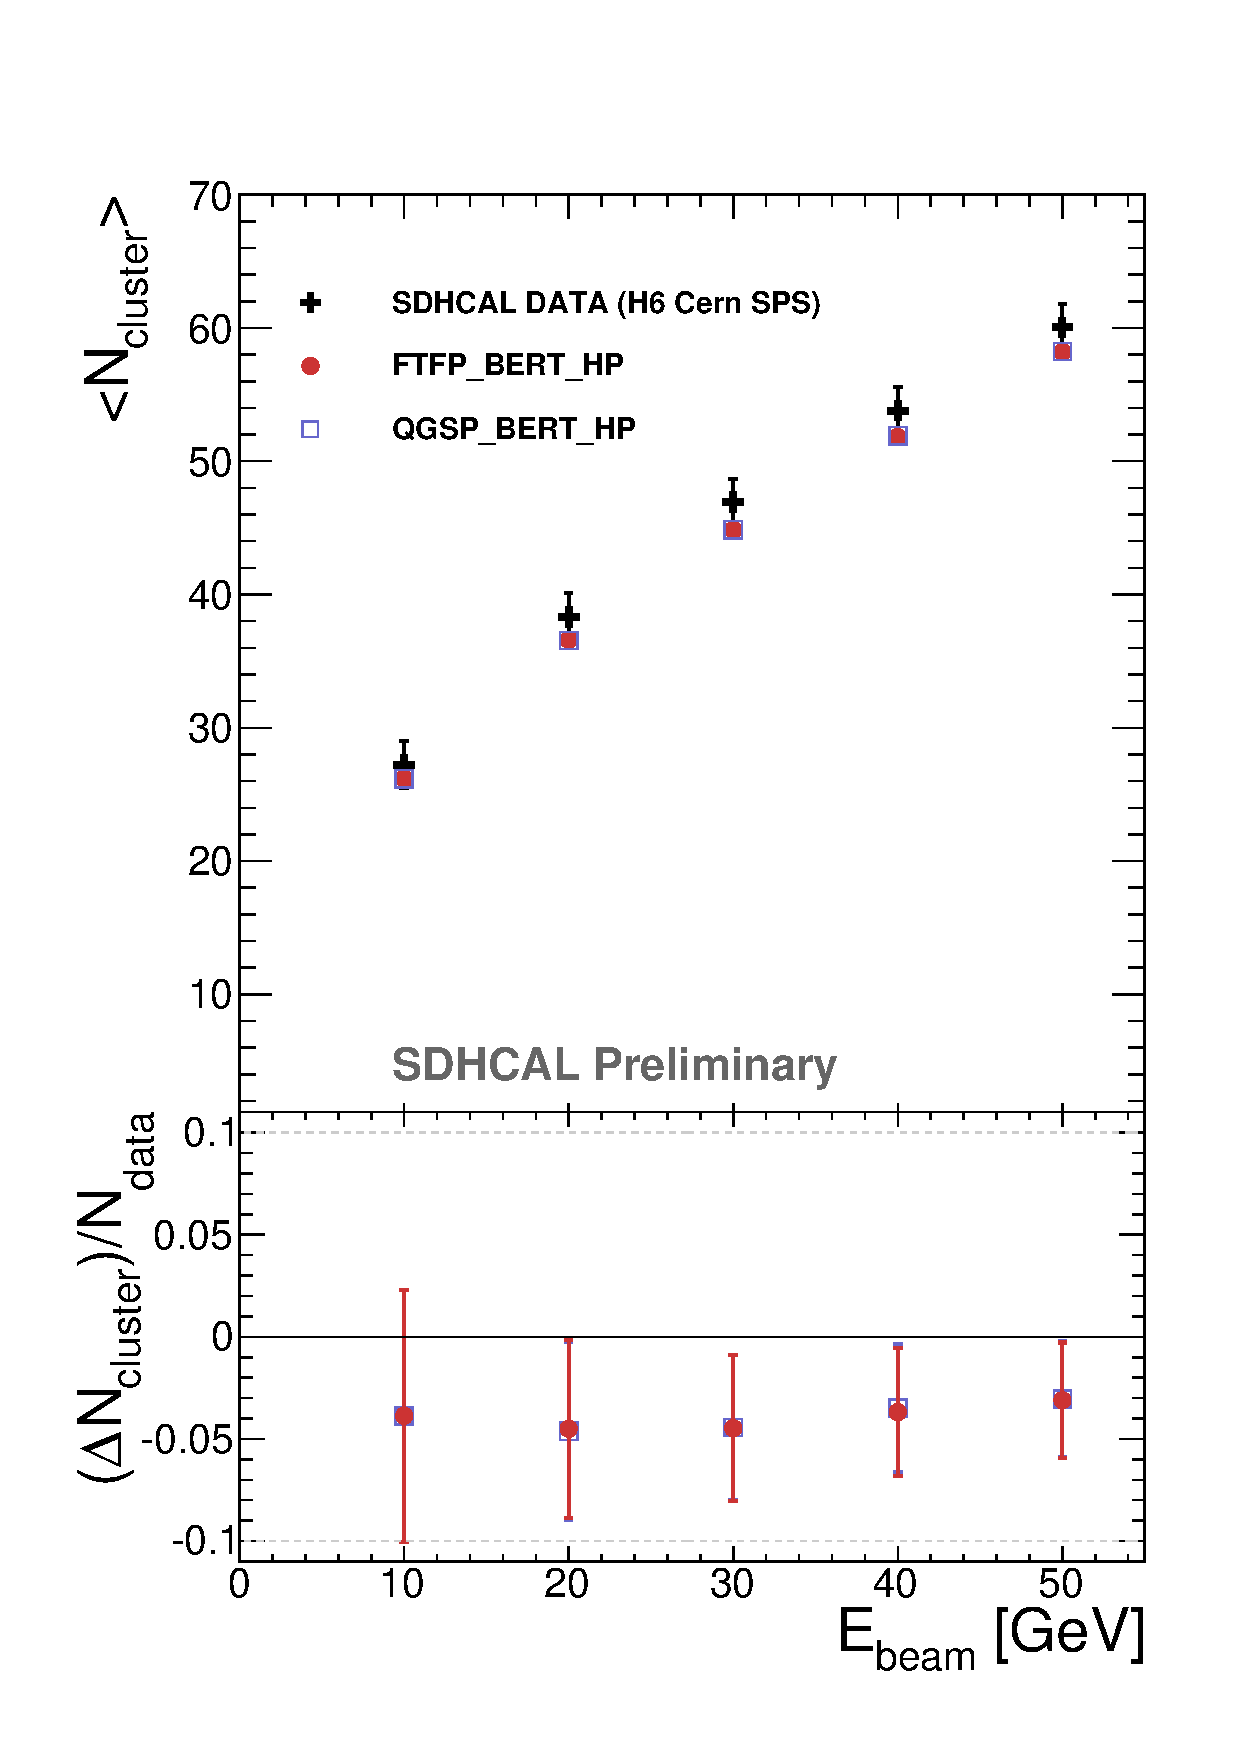
\includegraphics[width=.5\textwidth]{Shower/figs/NCLUSTERELECTRON.pdf}
%%   \caption{Moyenne du nombre de groupes de coups et déviation relative pour des gerbes électromagnétiques en fonction de l'énergie du faisceau.}
%% \end{figure}
%% \chapter{}
%% \label{app.longi}
%% \begin{figure}[!ht]
%%   \centering
%%   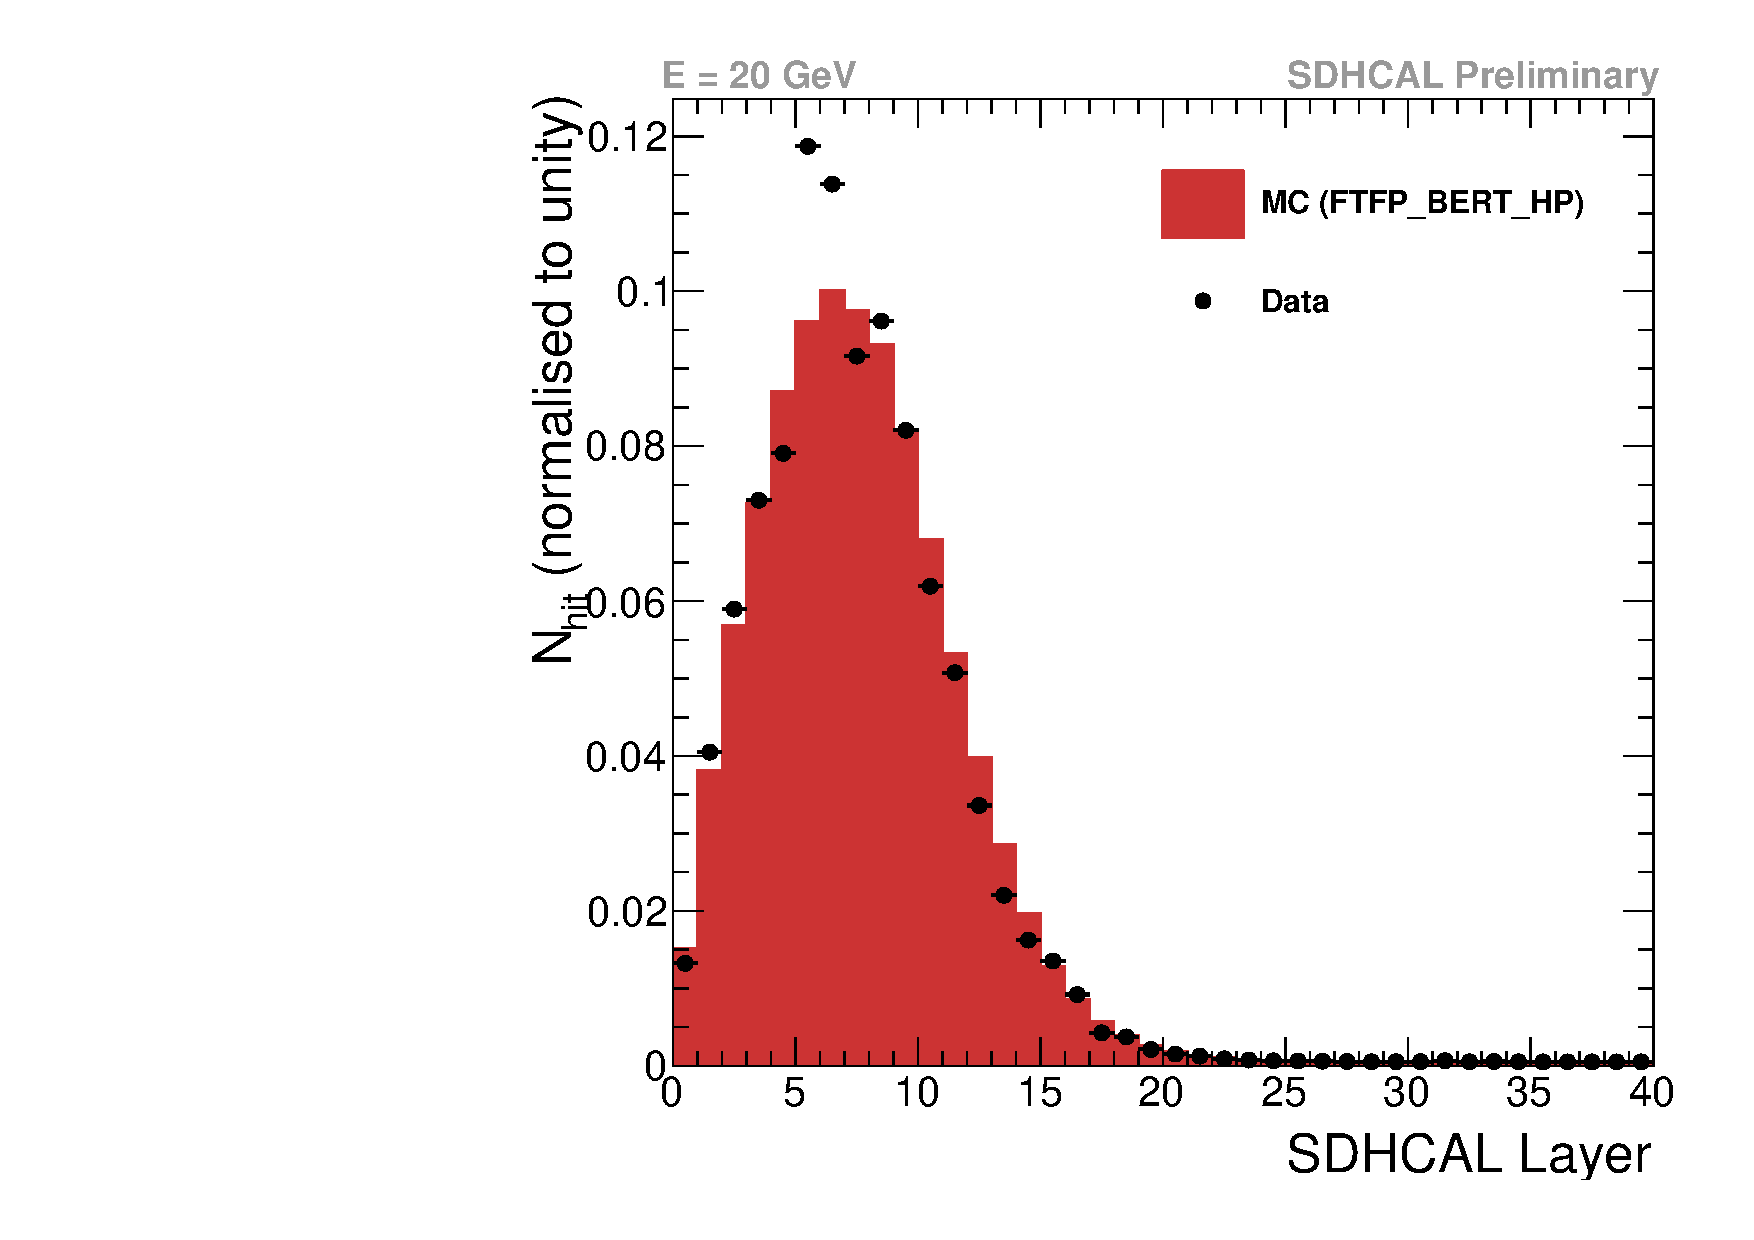
\includegraphics[width=.40\textwidth]{Shower/figs/longiProf_e-_20GeV_AugSep2012.pdf}
%%   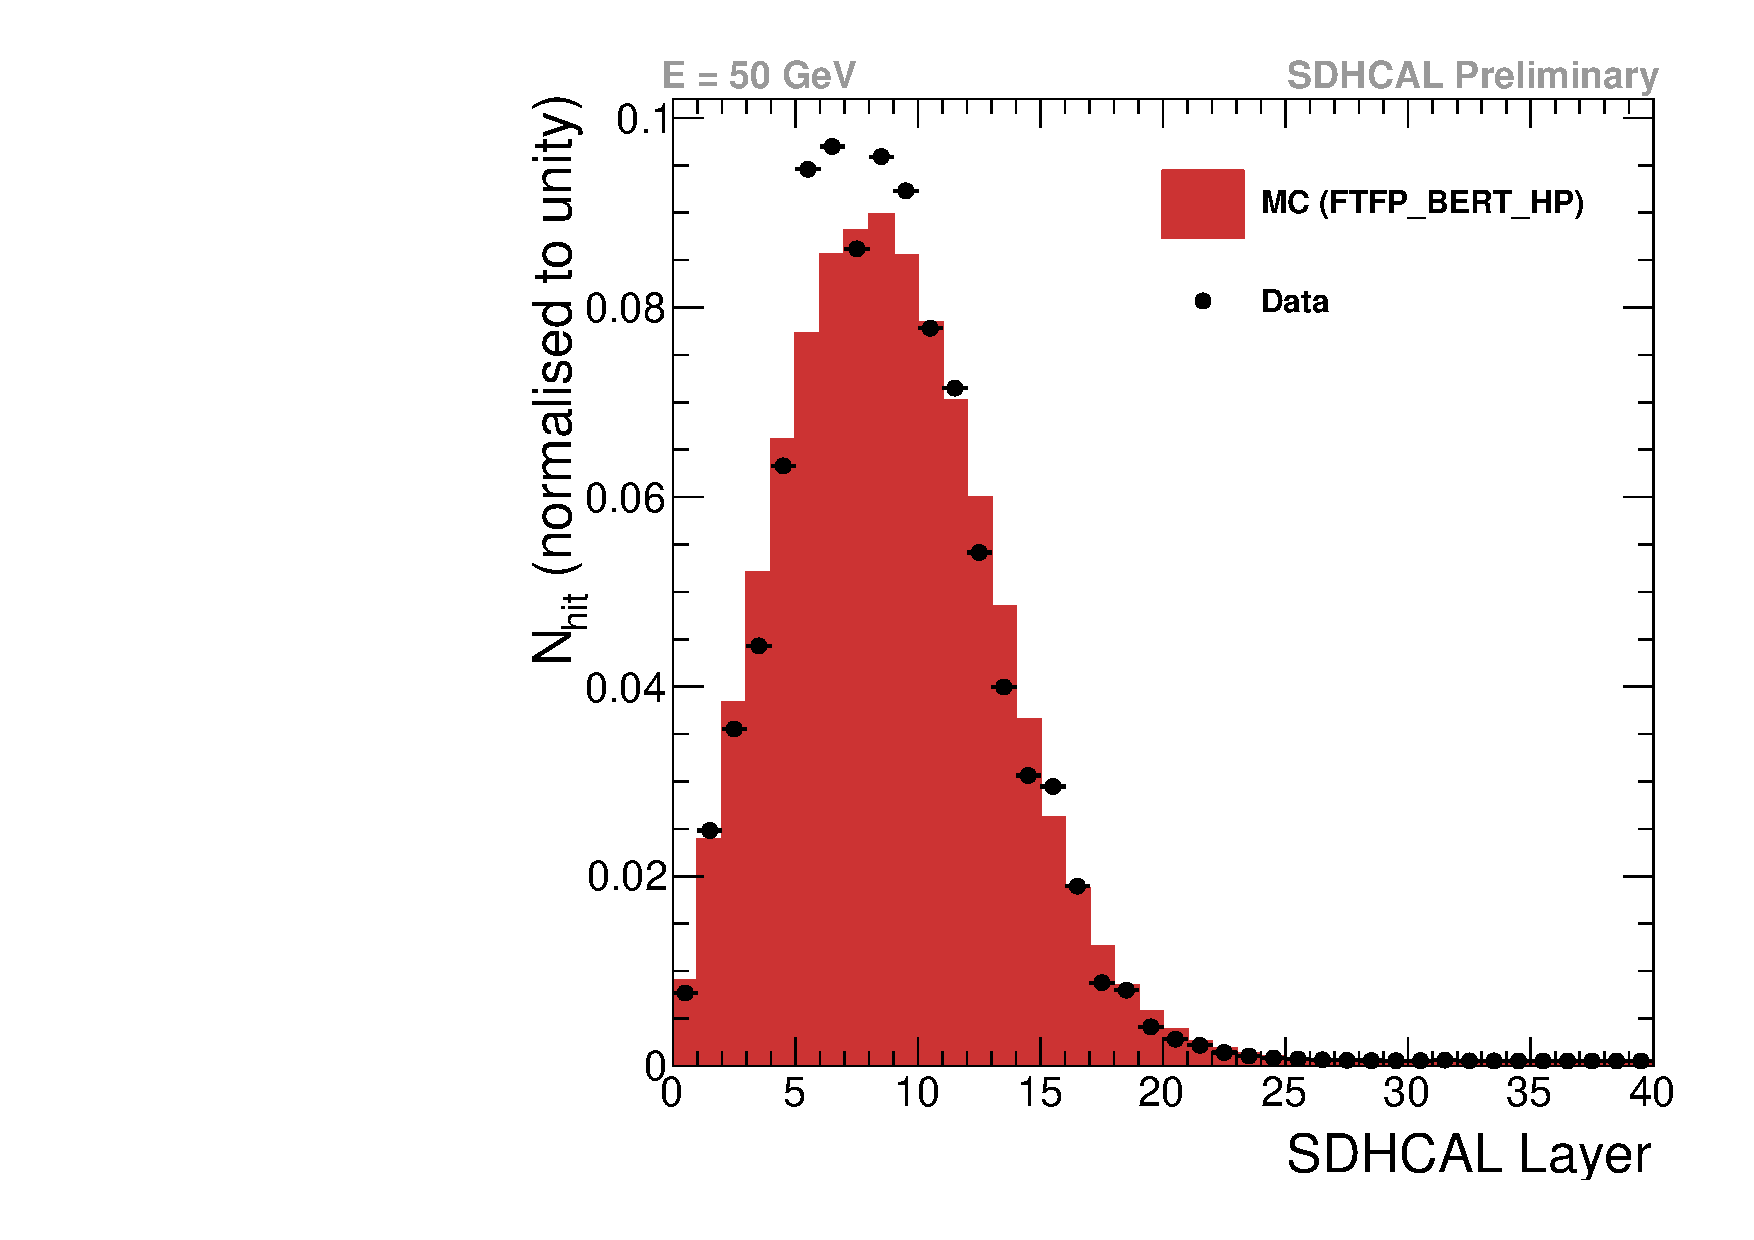
\includegraphics[width=.40\textwidth]{Shower/figs/longiProf_e-_50GeV_AugSep2012.pdf}
%%   \caption{Profil longitudinal de gerbes électromagnétiques à 20 (à gauche) et 50 $GeV$ (à droite) pour les données (cercles noirs) et une simulation réalisée avec liste physique FTFP\_BERT\_HP (histogramme plein).}
%%   \label{fig.longi_e-}
%% \end{figure}
%% \begin{figure}[!ht]
%%   \centering
%%   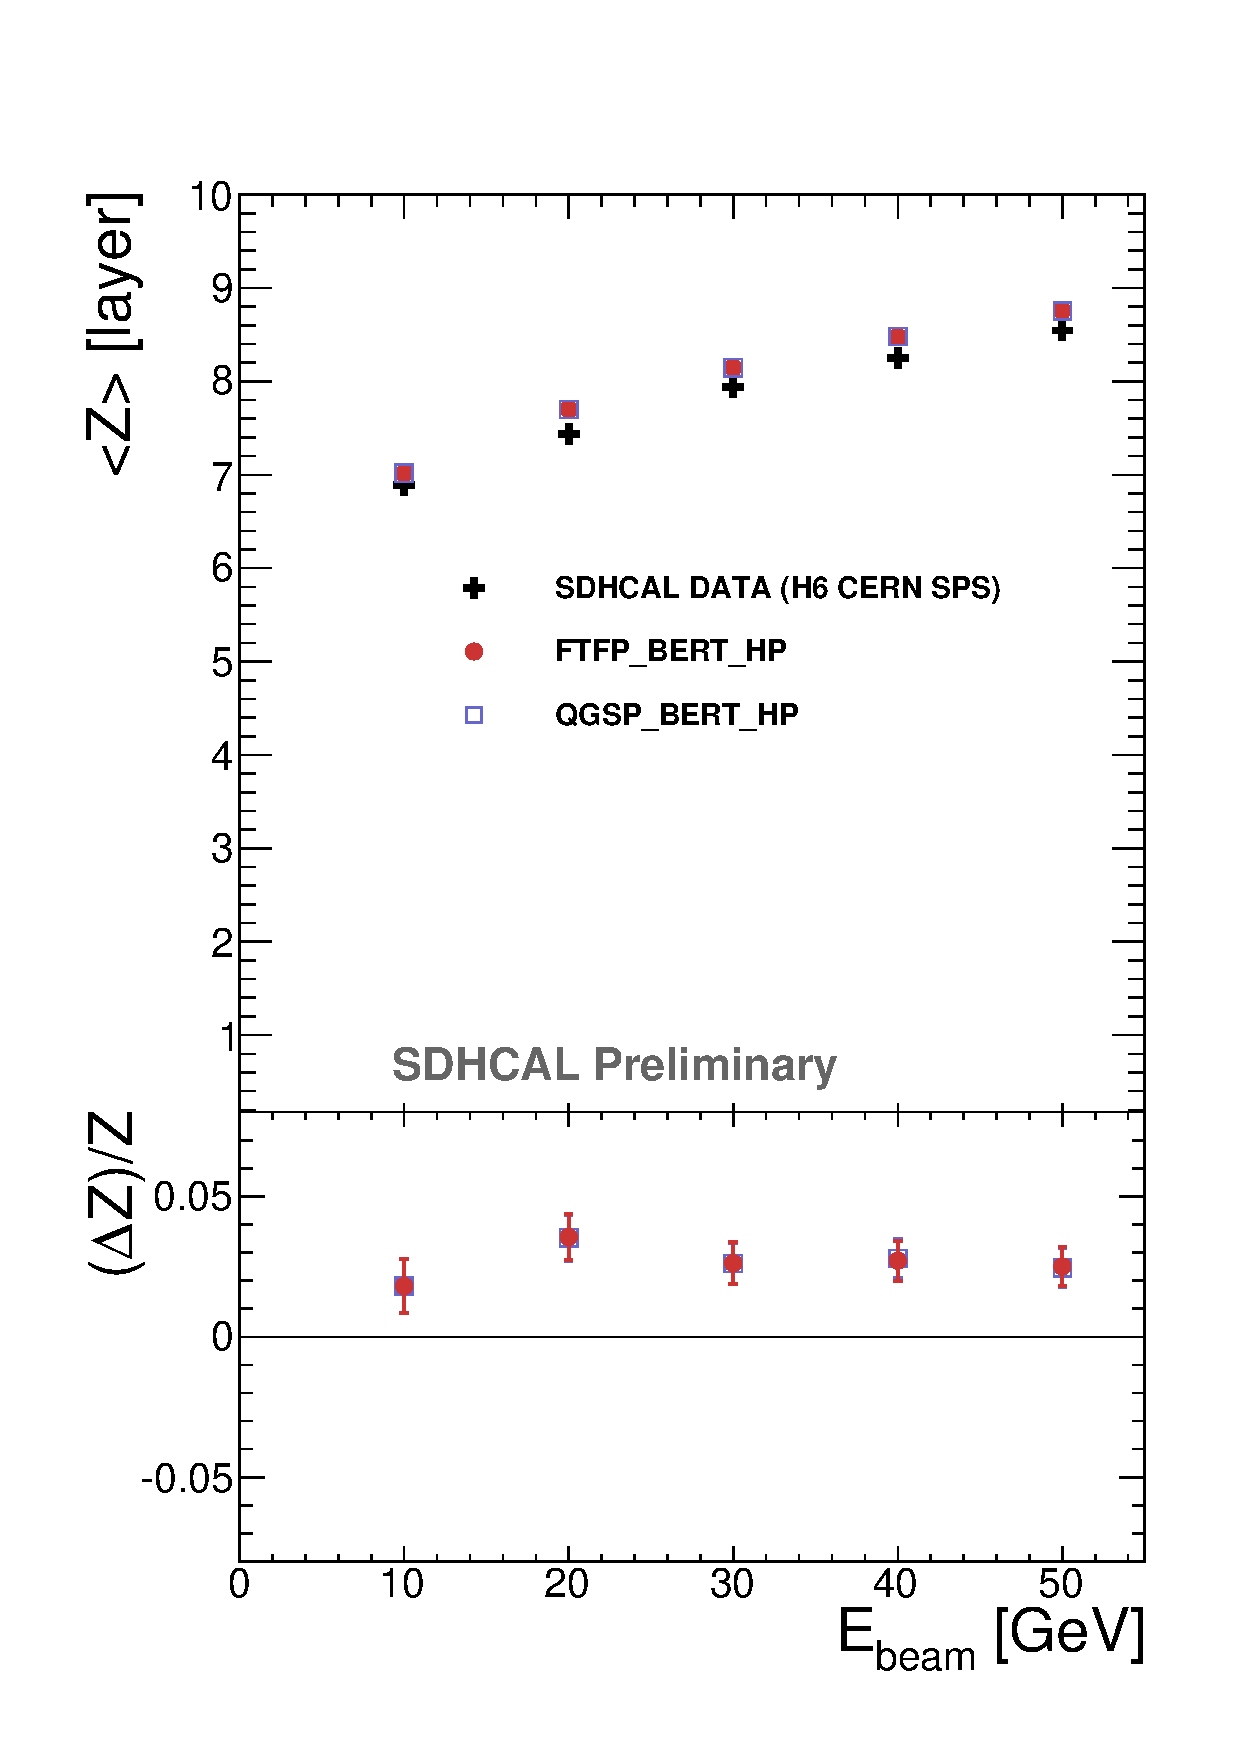
\includegraphics[width=.4\textwidth]{Shower/figs/LONGIELECTRON.pdf}
%%   \caption{Valeur moyenne et déviation relative du profil longitudinal pour des gerbes électromagnétiques en fonction de l'énergie du faisceau.}
%%   \label{fig.longi_e-_ebeam}
%% \end{figure}
\chapter{}
\label{app.radial}
\begin{figure}[!ht]
  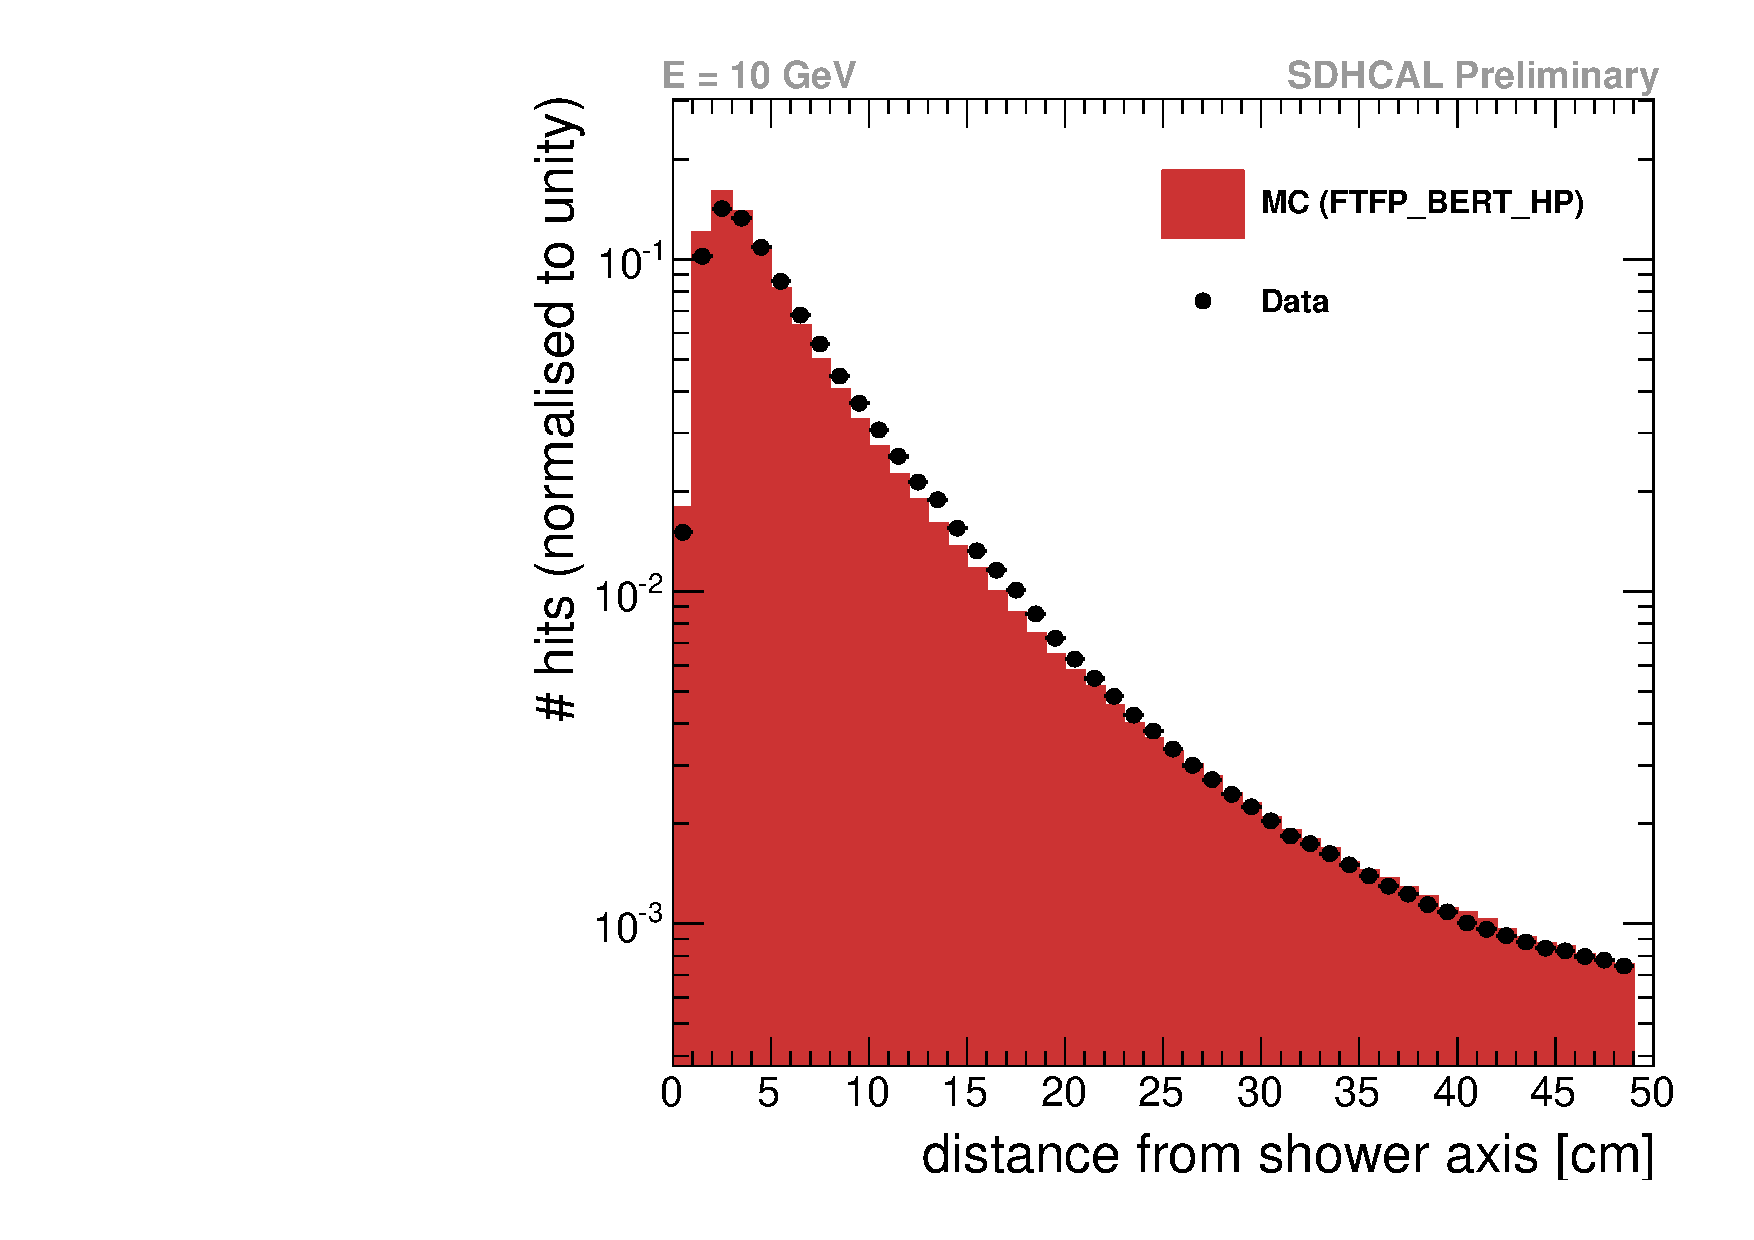
\includegraphics[width=.32\textwidth]{Shower/figs/radProfLog_pi-_10GeV_ftfp_bert_hp.pdf}
  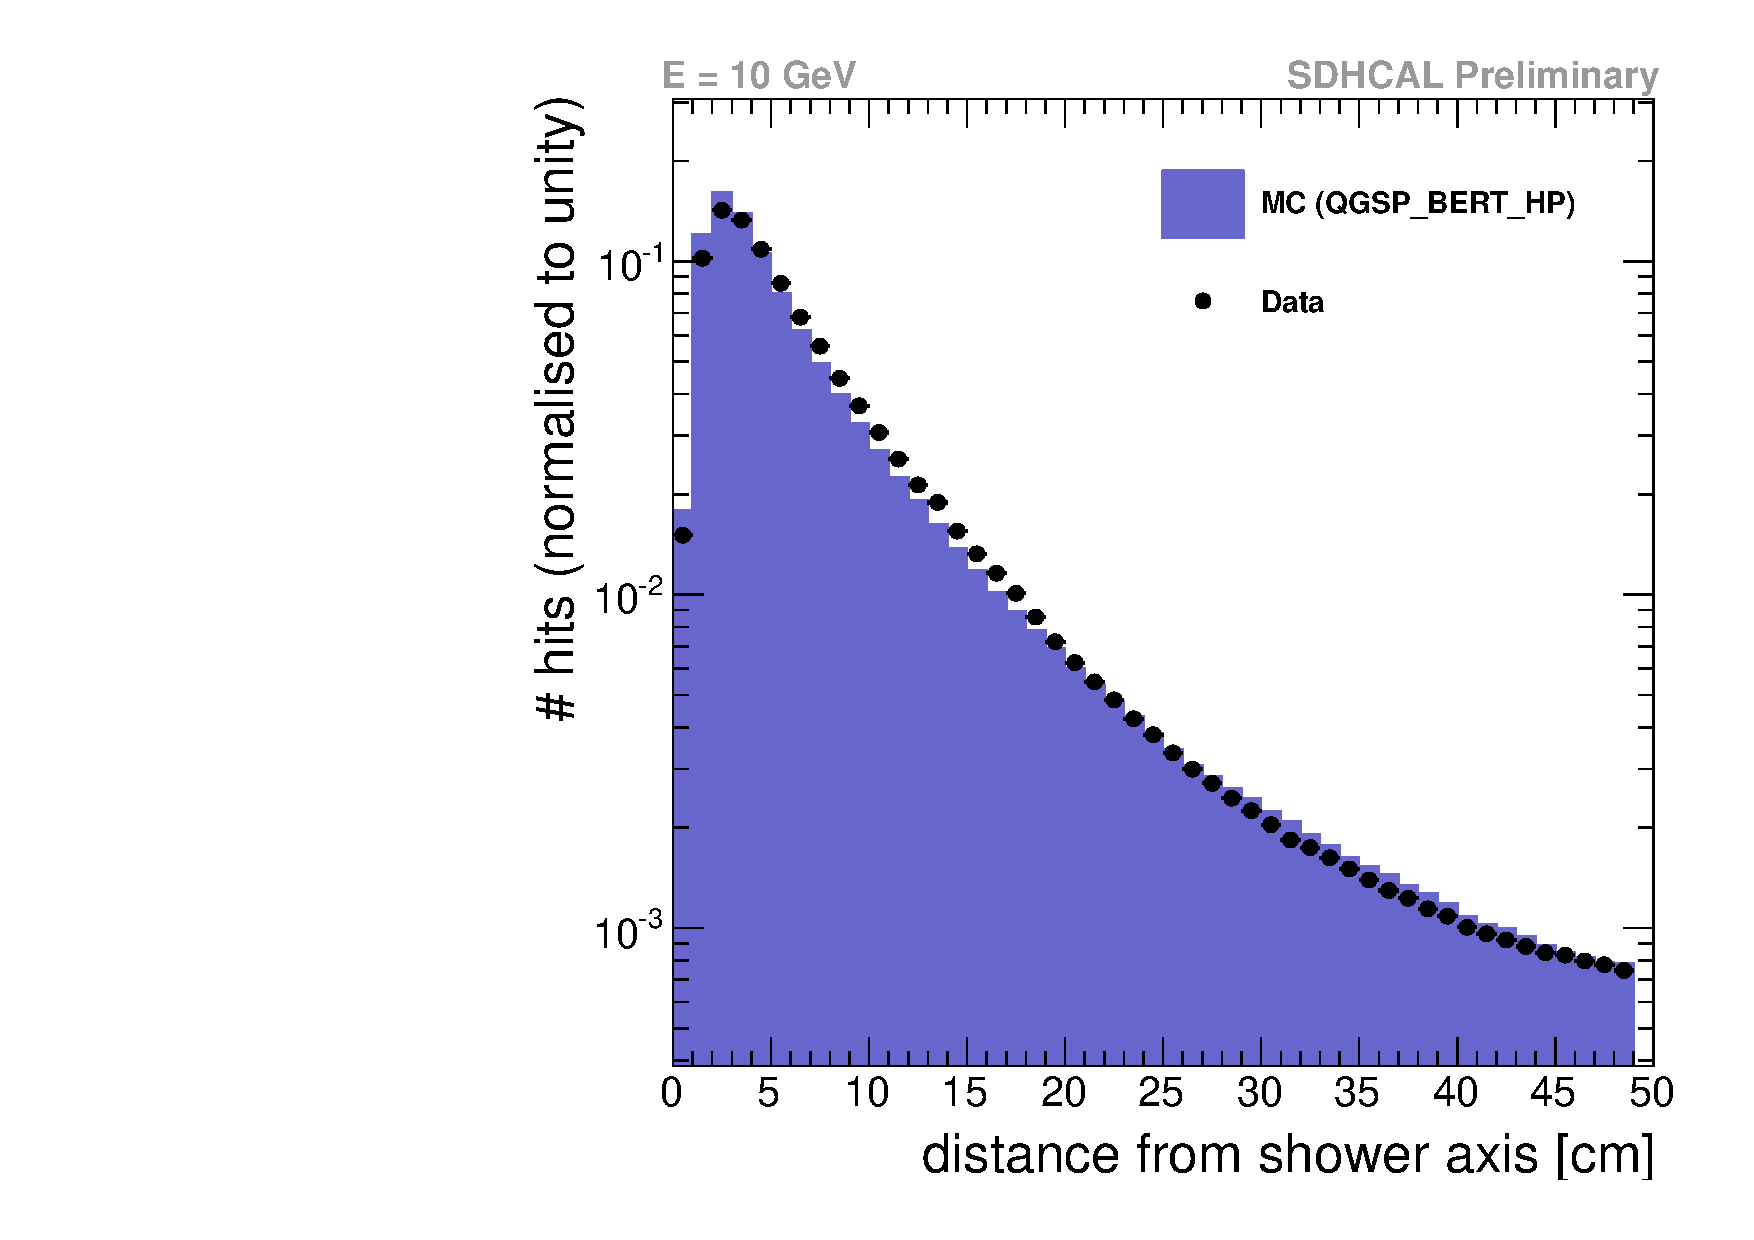
\includegraphics[width=.32\textwidth]{Shower/figs/radProfLog_pi-_10GeV_qgsp_bert_hp.pdf}
  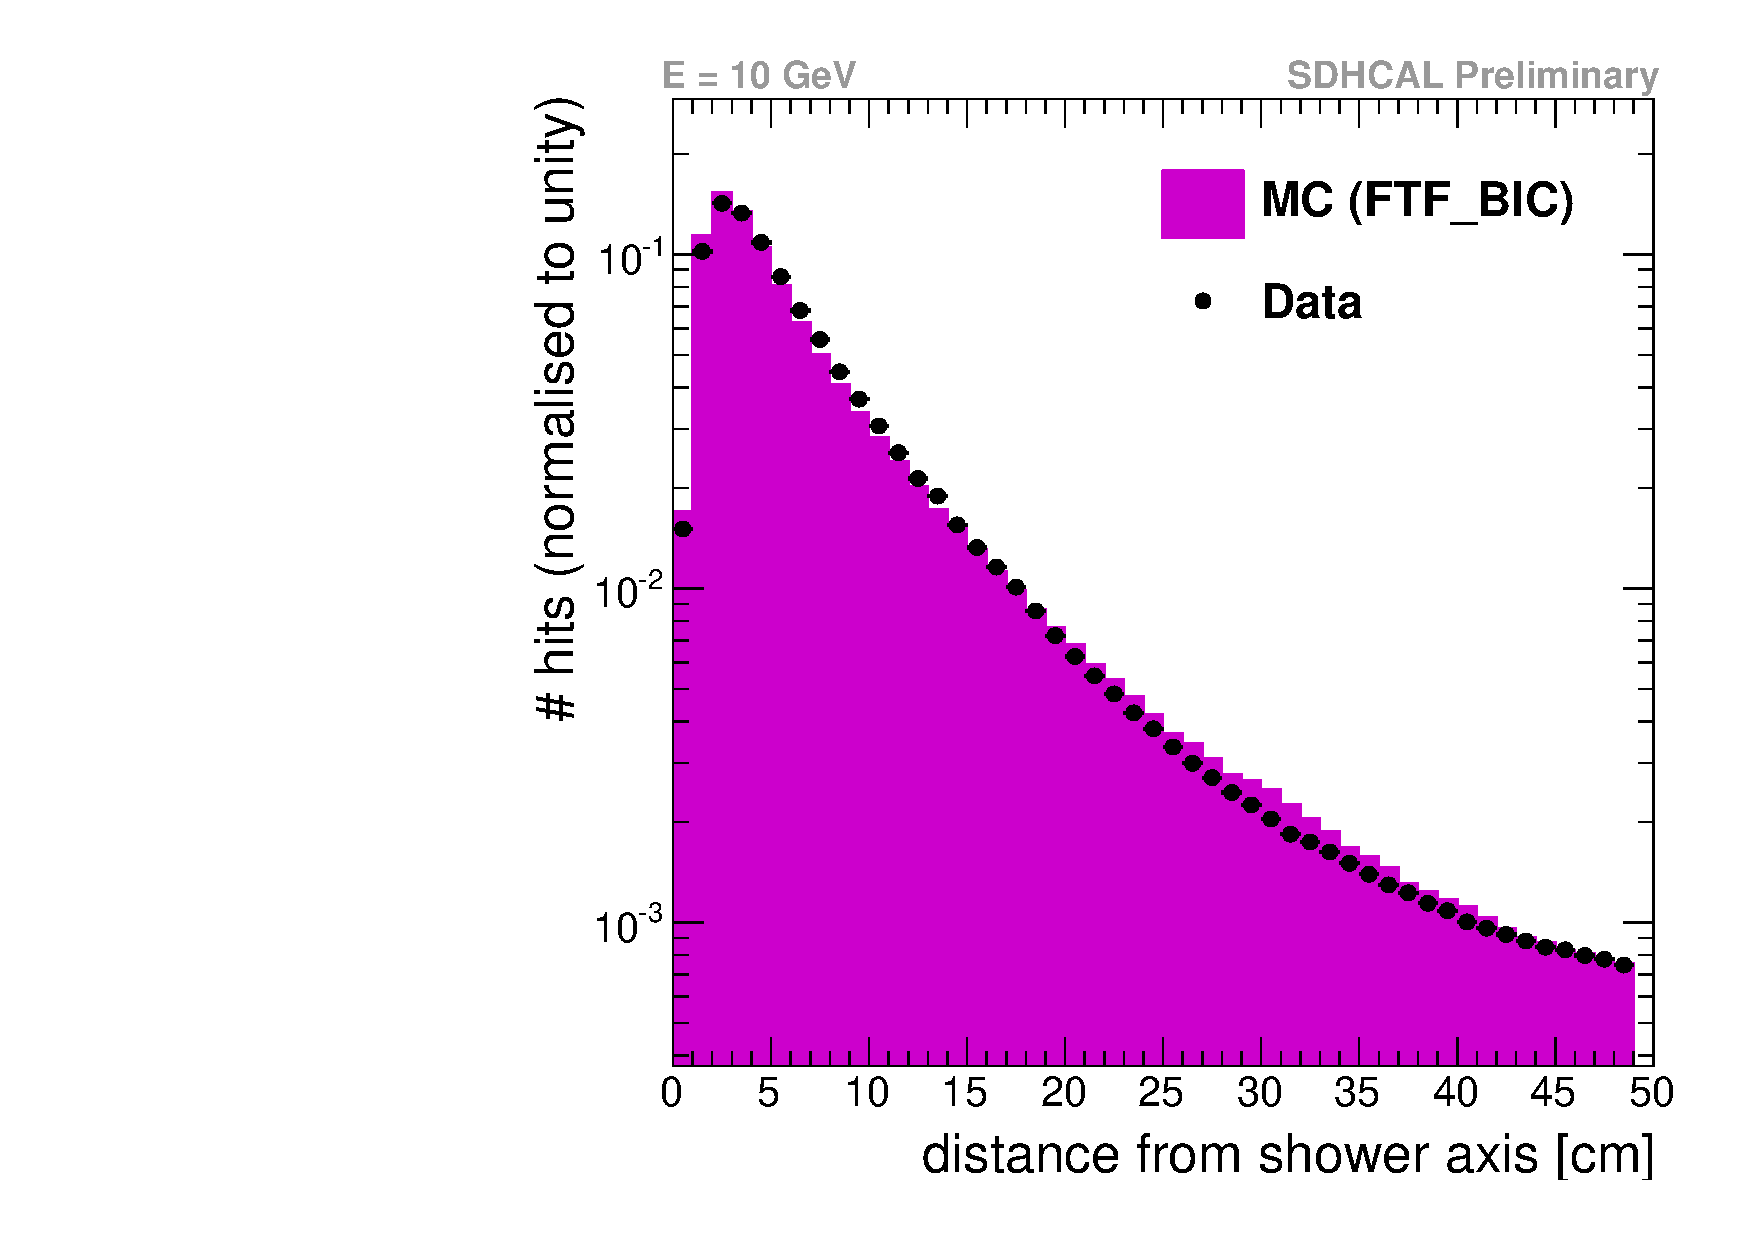
\includegraphics[width=.32\textwidth]{Shower/figs/radProfLog_pi-_10GeV_ftf_bic.pdf}  \\
  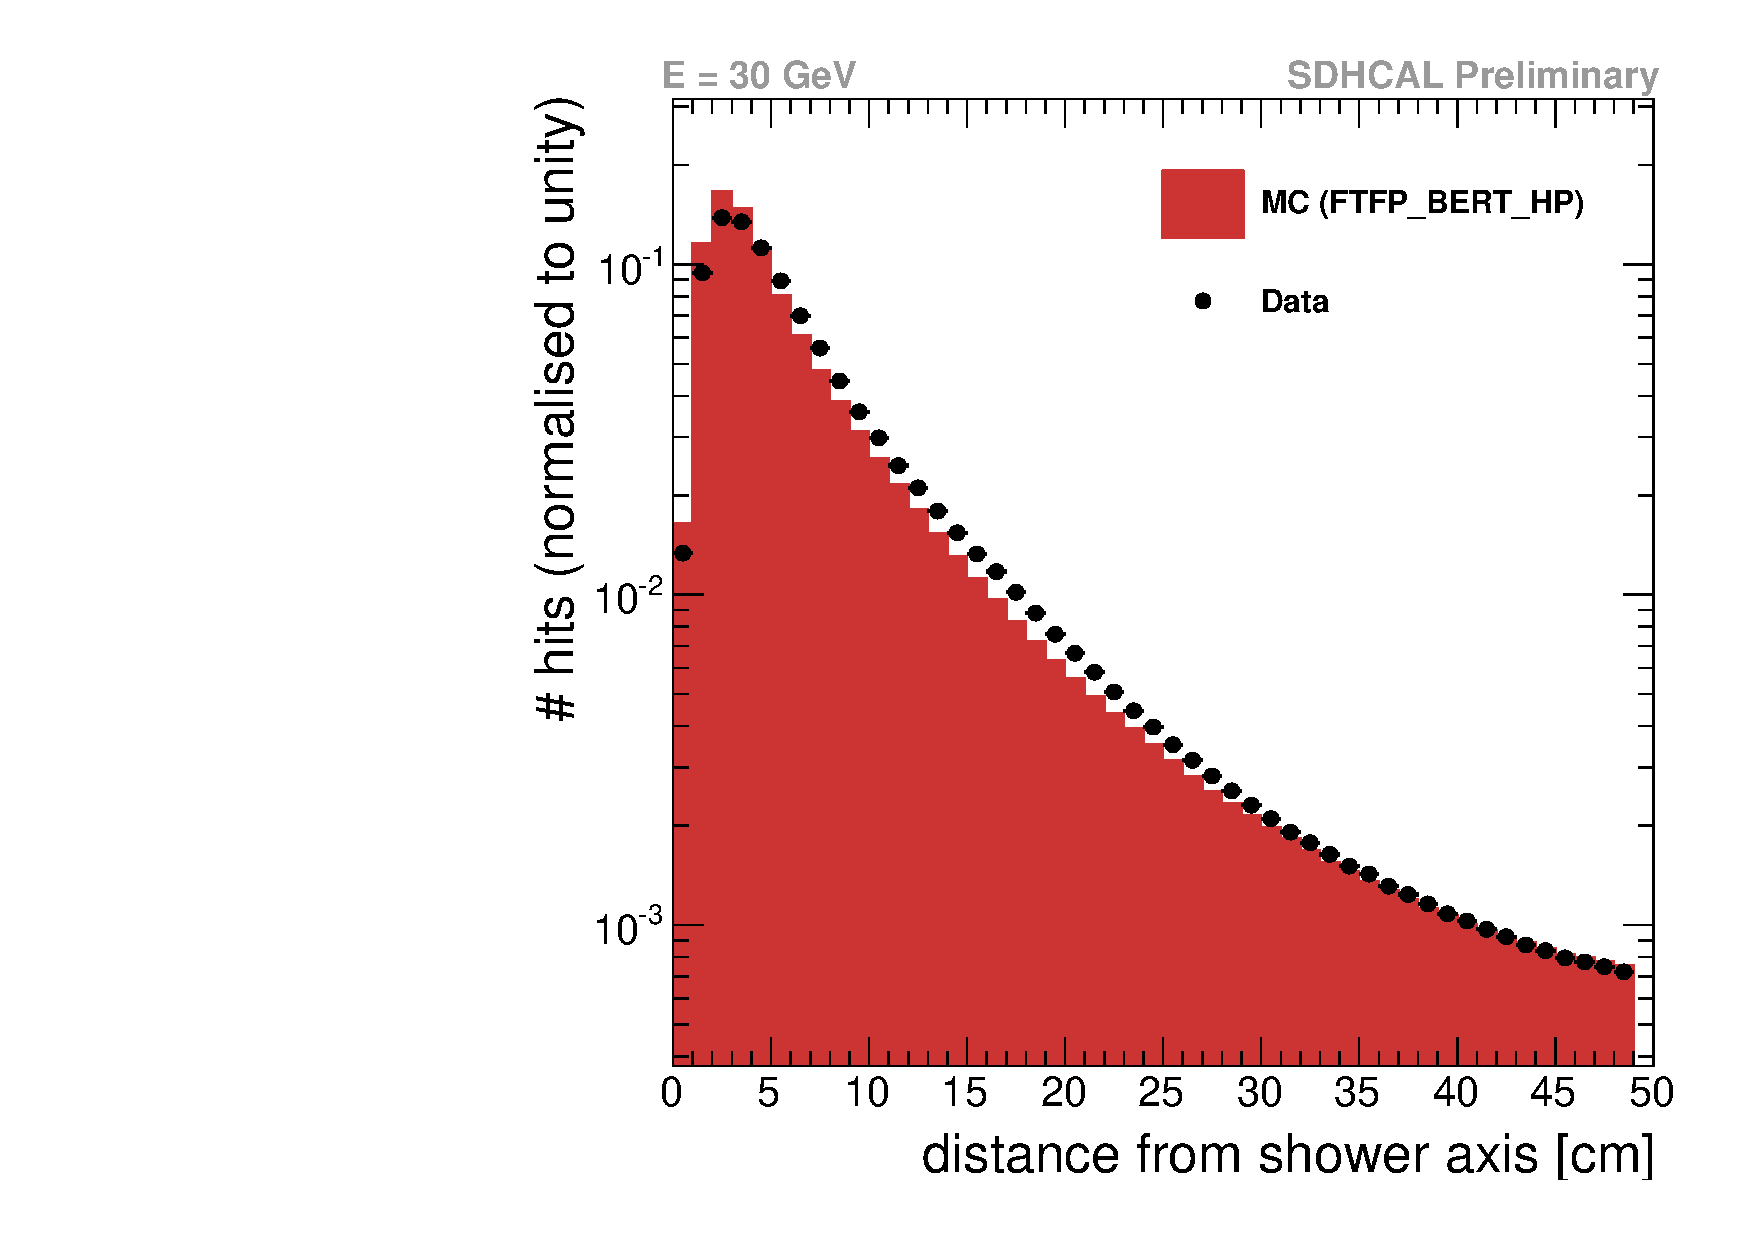
\includegraphics[width=.32\textwidth]{Shower/figs/radProfLog_pi-_30GeV_ftfp_bert_hp.pdf}
  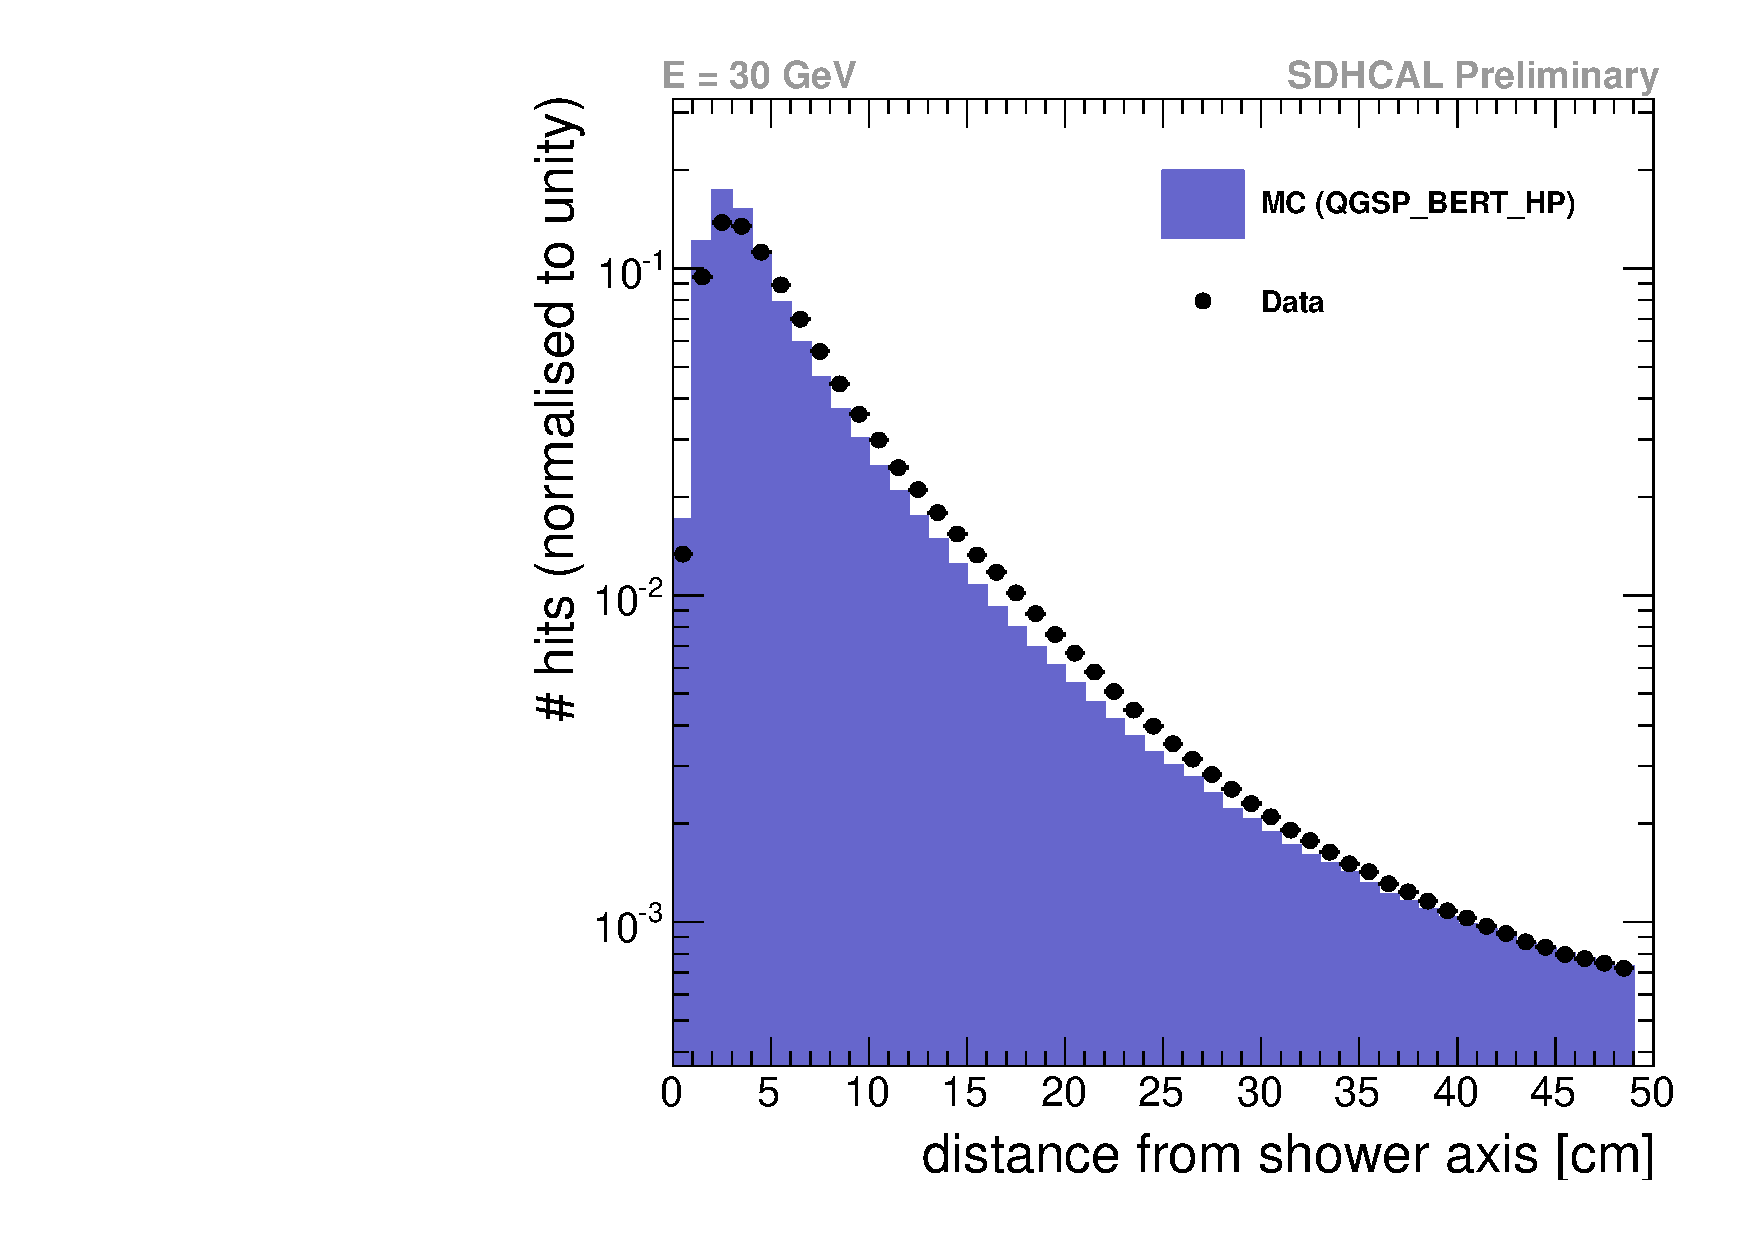
\includegraphics[width=.32\textwidth]{Shower/figs/radProfLog_pi-_30GeV_qgsp_bert_hp.pdf}
  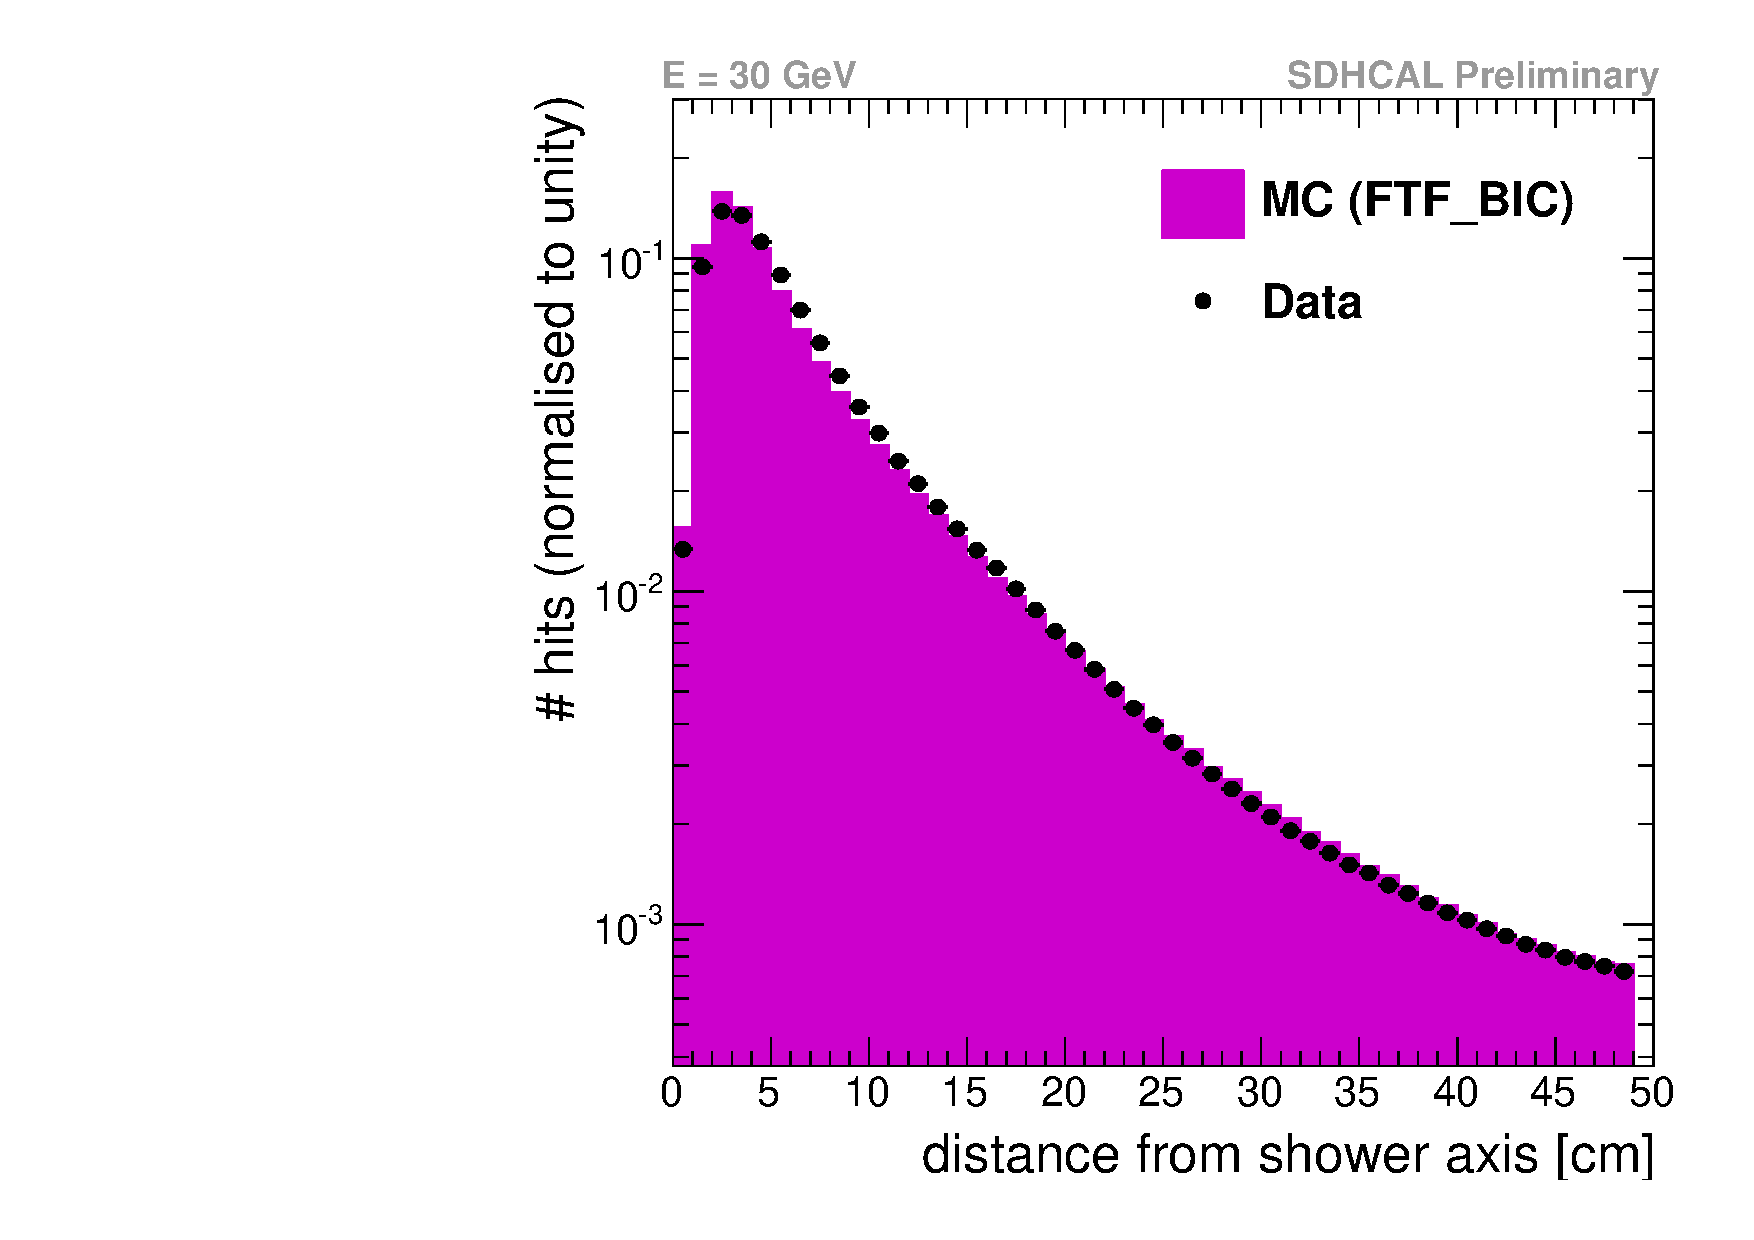
\includegraphics[width=.32\textwidth]{Shower/figs/radProfLog_pi-_30GeV_ftf_bic.pdf}  \\
  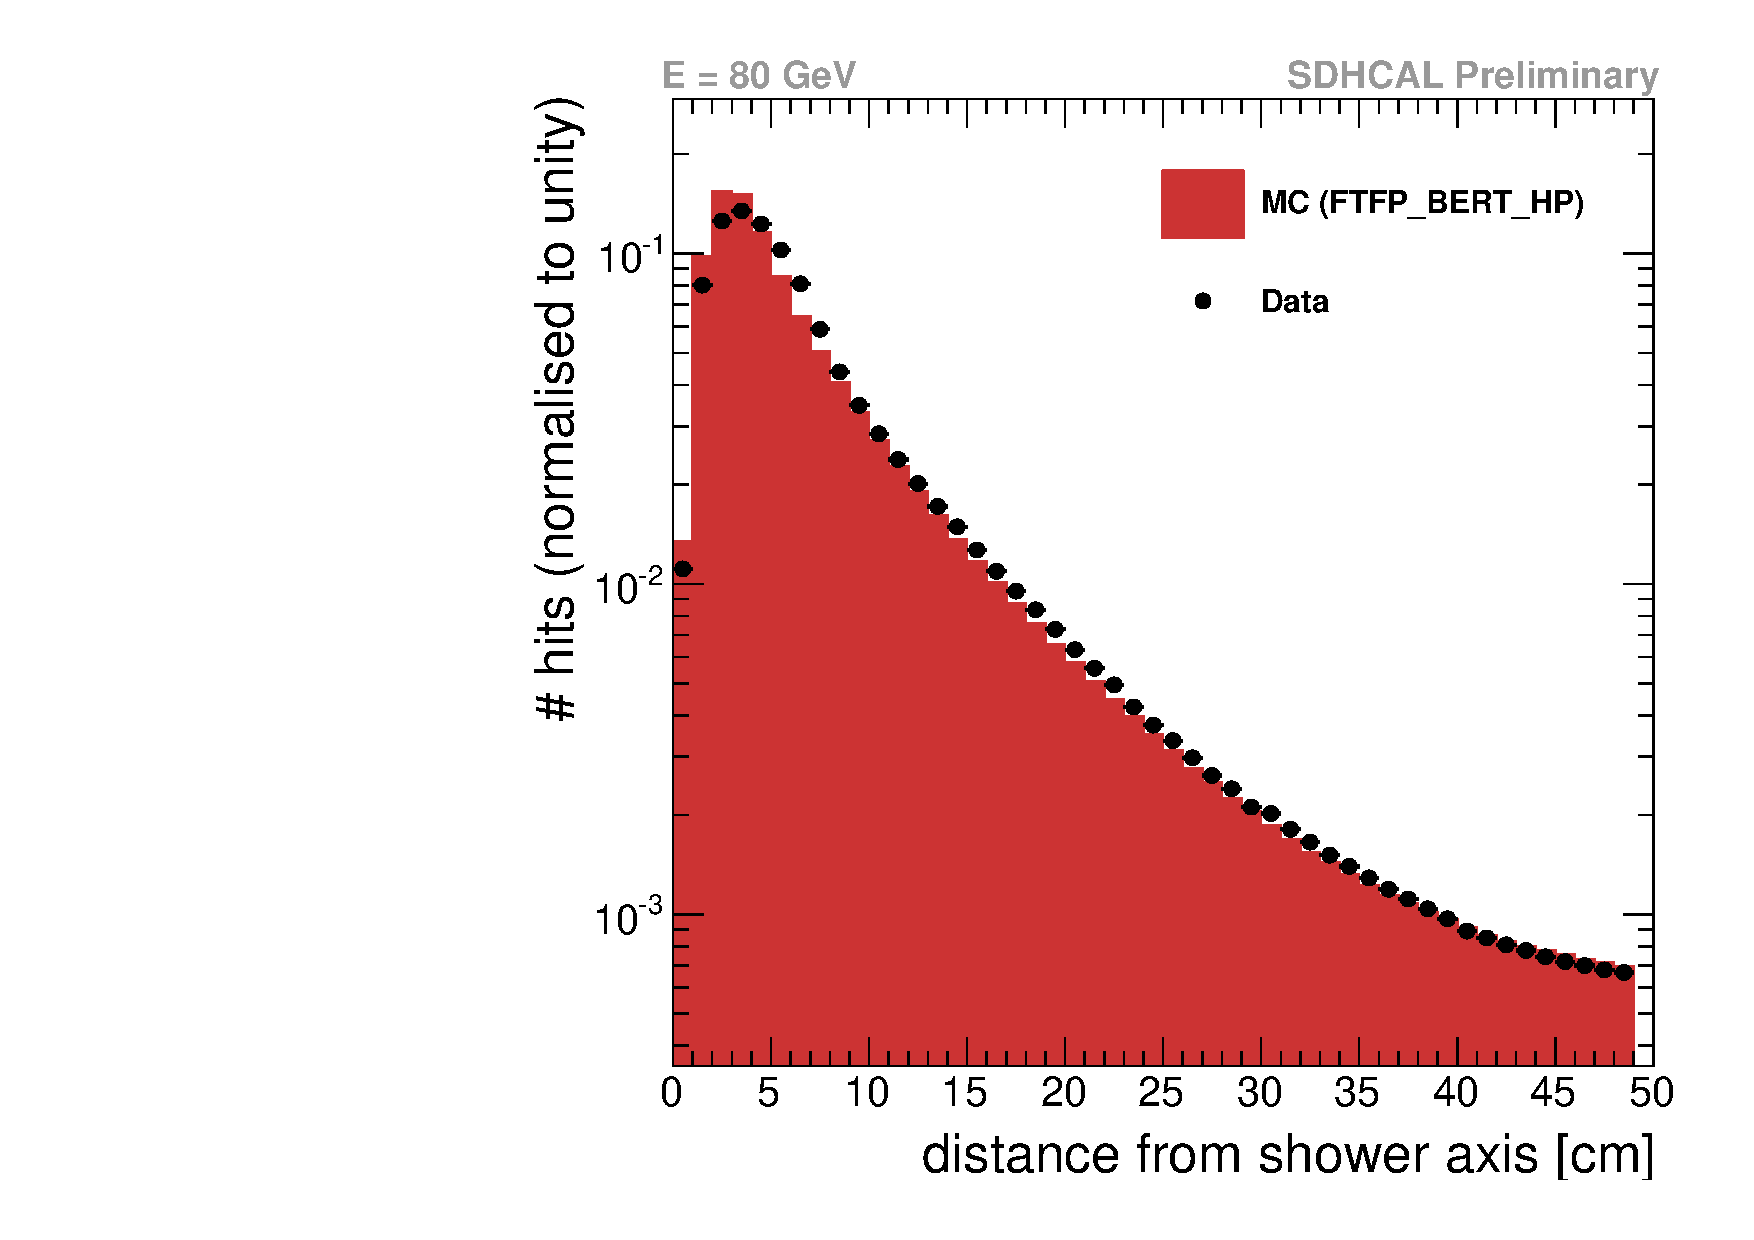
\includegraphics[width=.32\textwidth]{Shower/figs/radProfLog_pi-_80GeV_ftfp_bert_hp.pdf}
  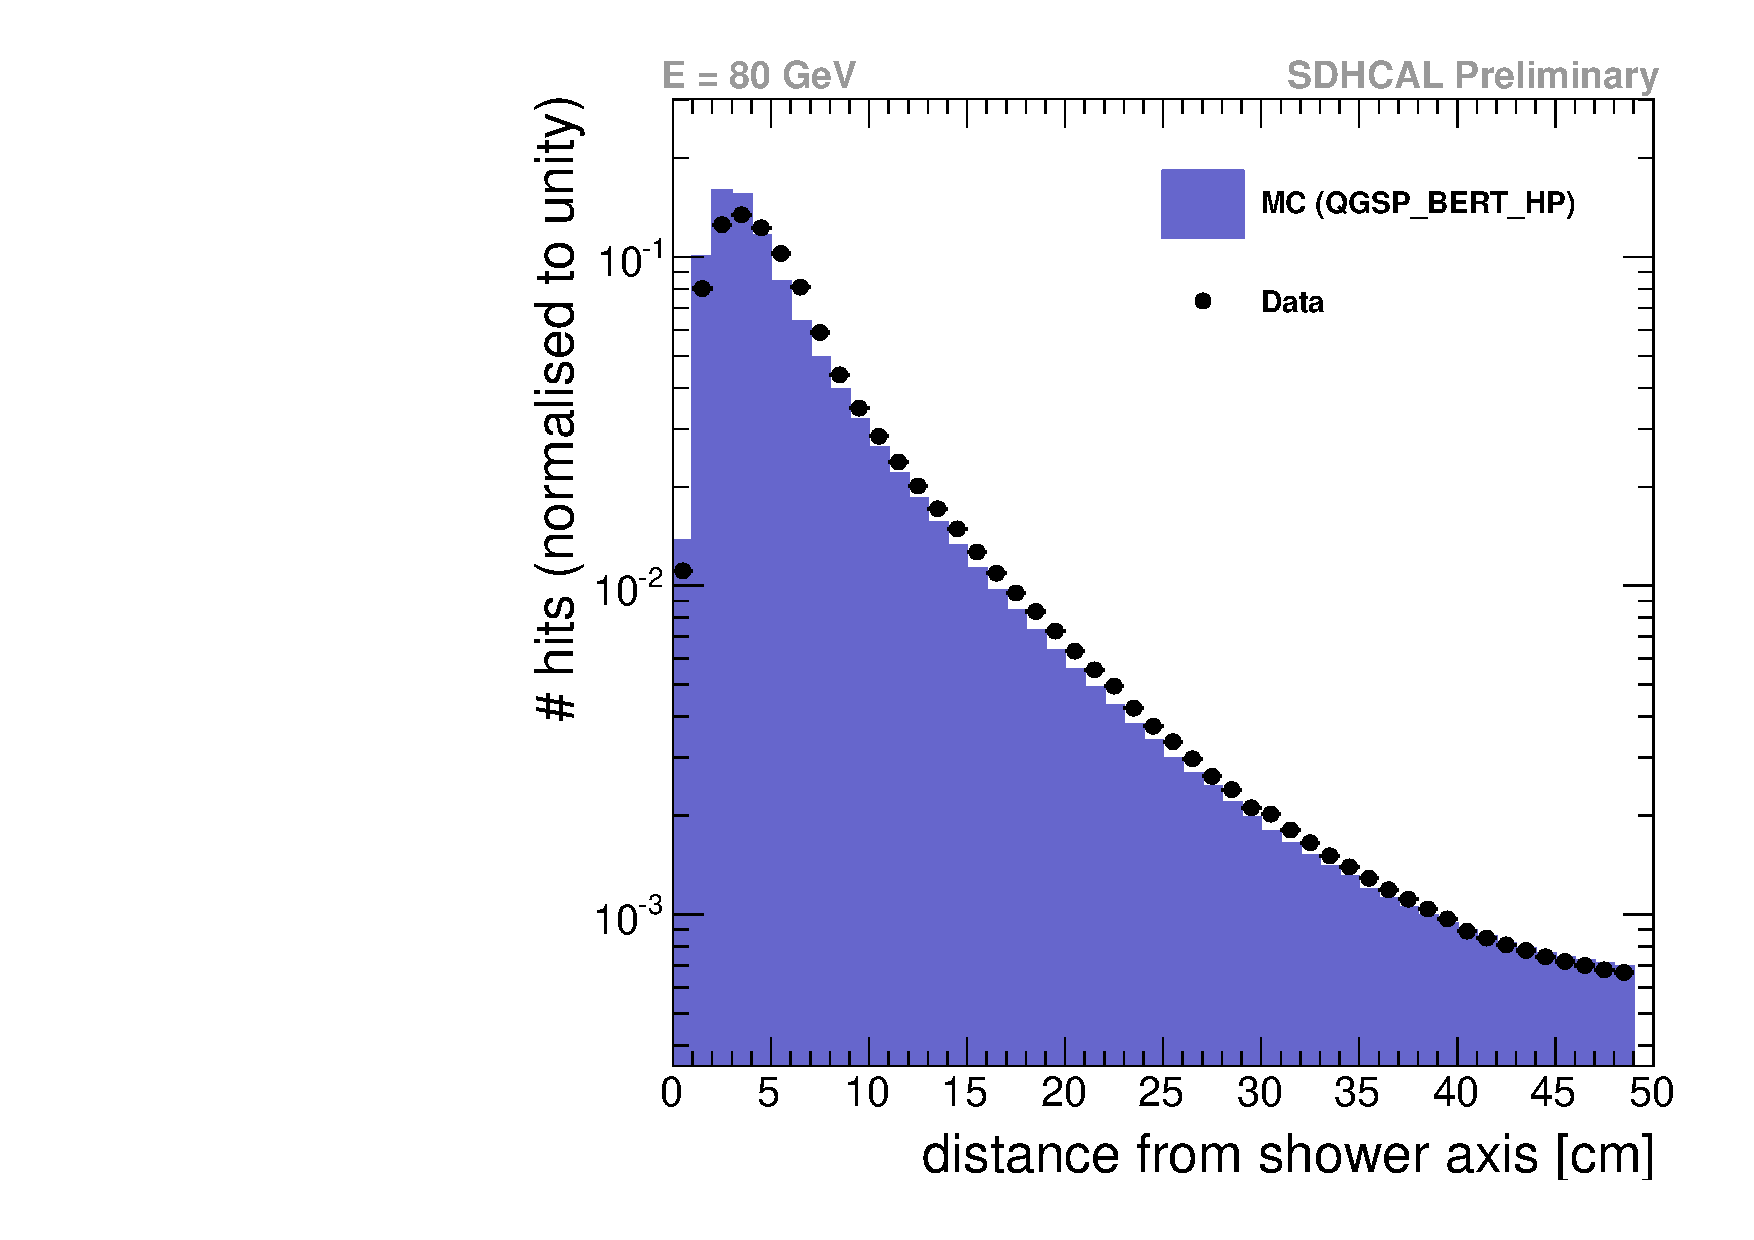
\includegraphics[width=.32\textwidth]{Shower/figs/radProfLog_pi-_80GeV_qgsp_bert_hp.pdf}
  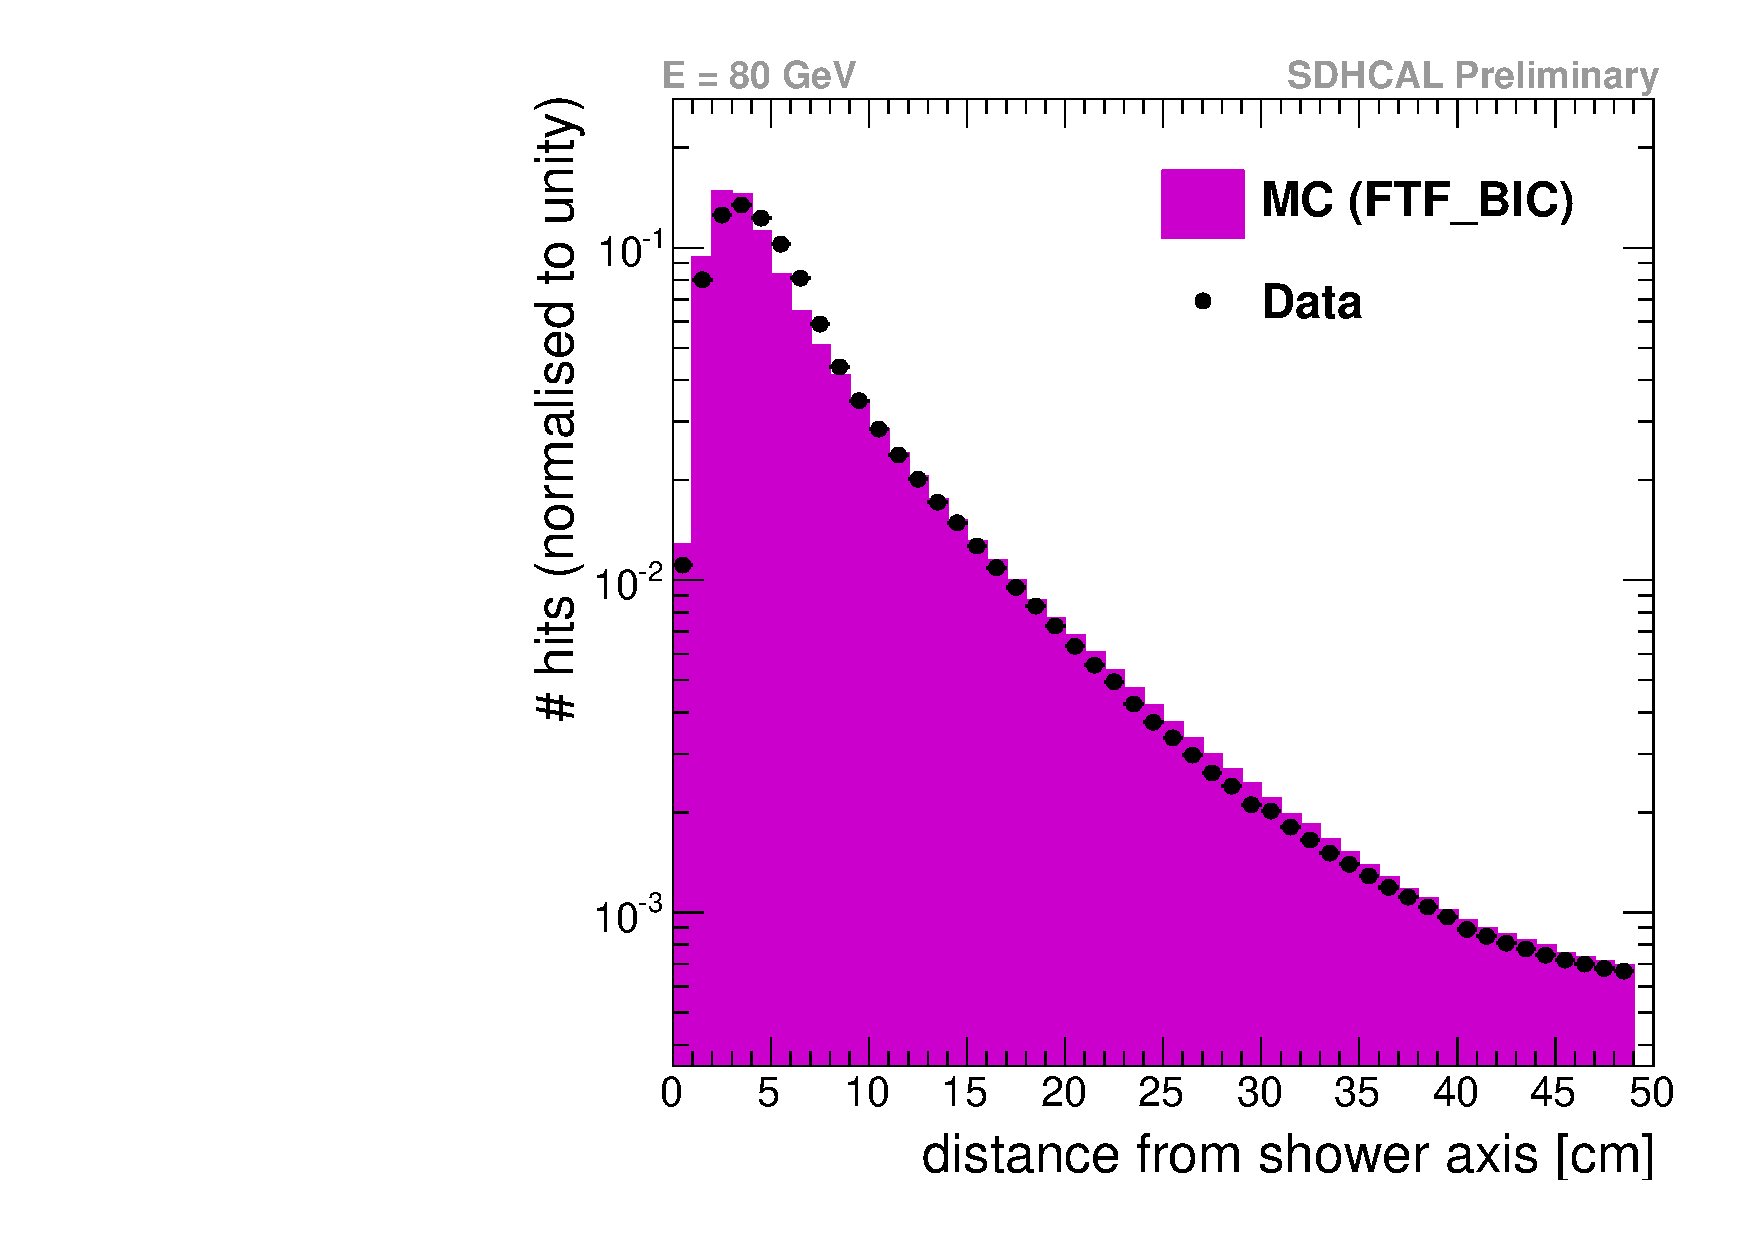
\includegraphics[width=.32\textwidth]{Shower/figs/radProfLog_pi-_80GeV_ftf_bic.pdf}
  \caption{Profile transversale pour des échantillons de pions de 10 GeV (en haut), de 30 GeV (au milieu) et de 80 GeV (en bas) pour les données et des simulation réalisée avec les listes FTFP\_BERT\_HP (à gauche), QGSP\_BERT\_HP (au centre) et FTF\_BIC (à droite). Les données sont représentées par des cercles noirs et la simulation par les histogrammes rouges. \label{fig.pi-radial_log}}
\end{figure}
%% \chapter{}
%% \label{app.radial_e-}
%% \begin{figure}[!ht]
%%   \centering
%%   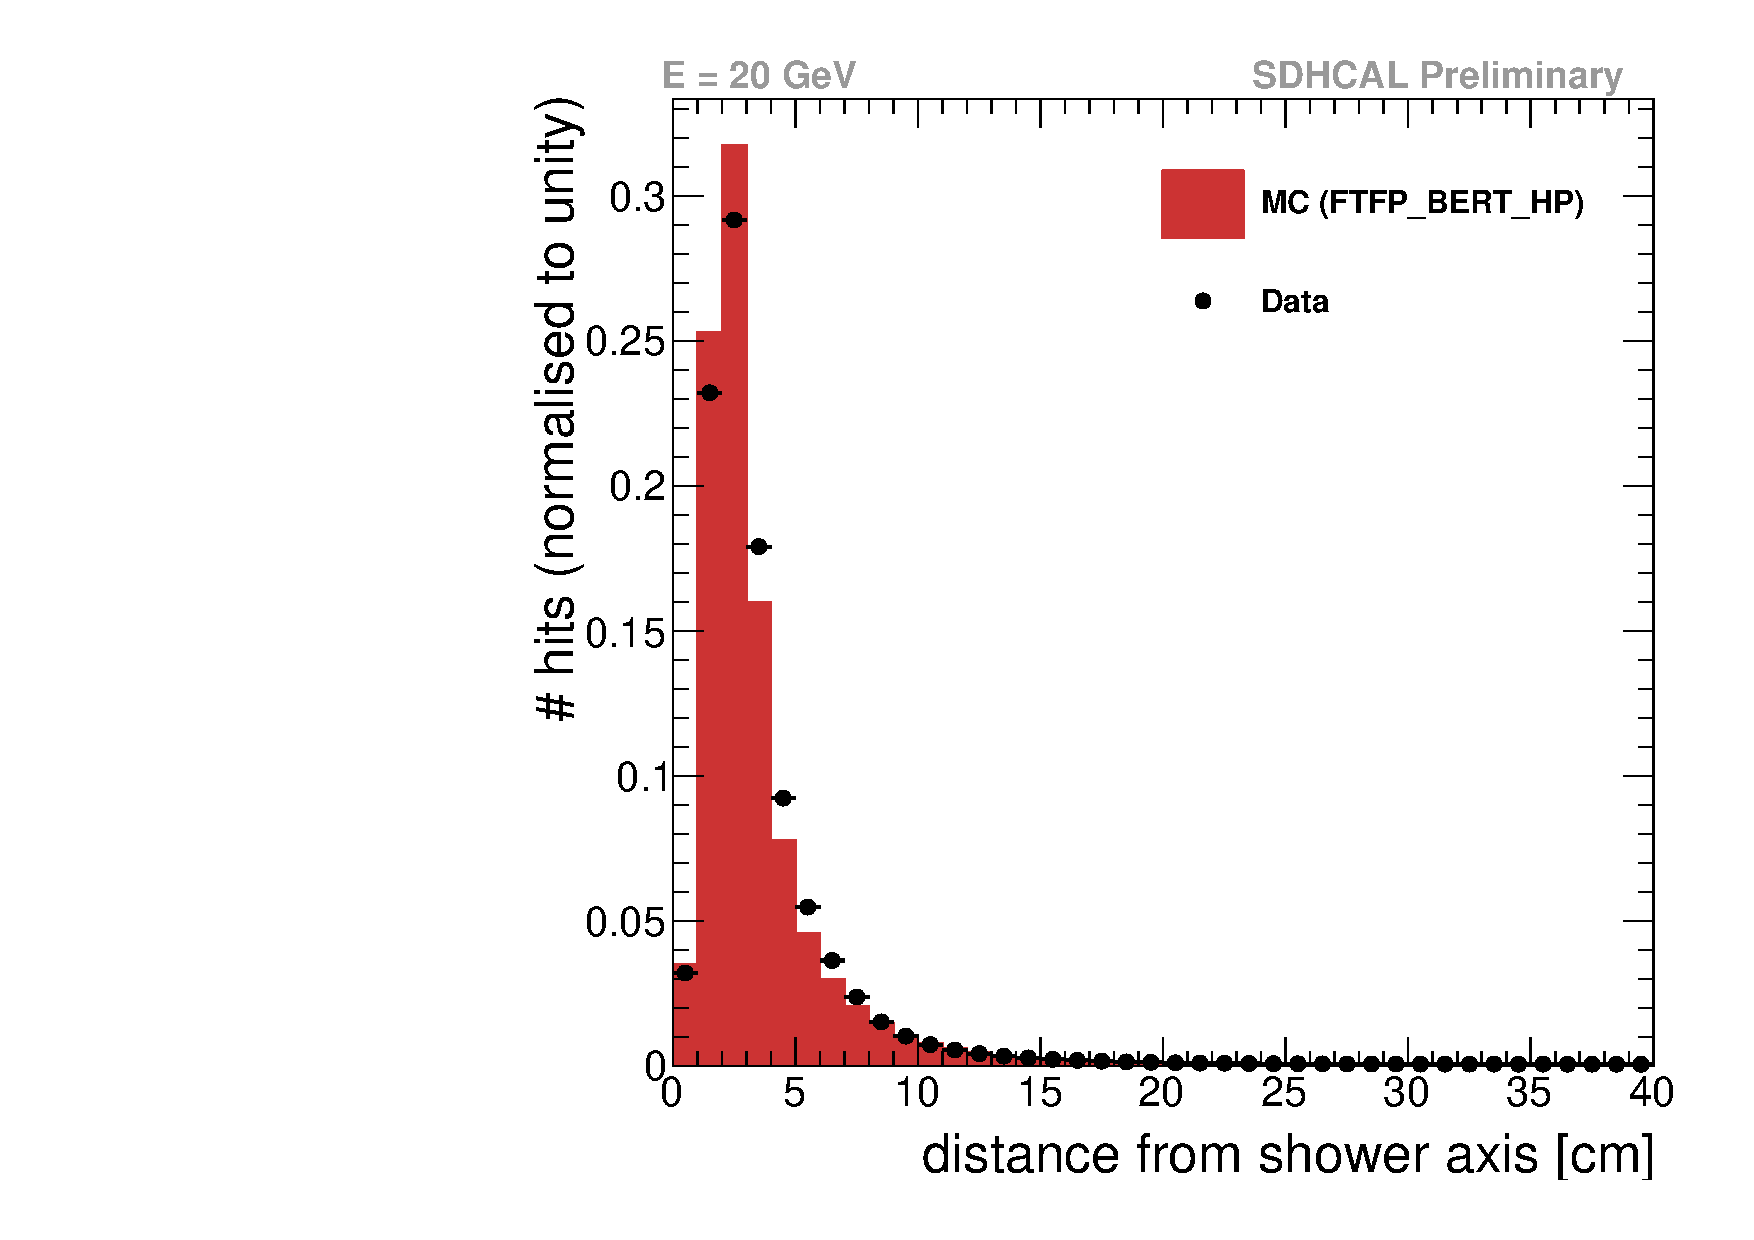
\includegraphics[width=.40\textwidth]{Shower/figs/radProf_e-_20GeV_AugSep2012.pdf
%% }
%%   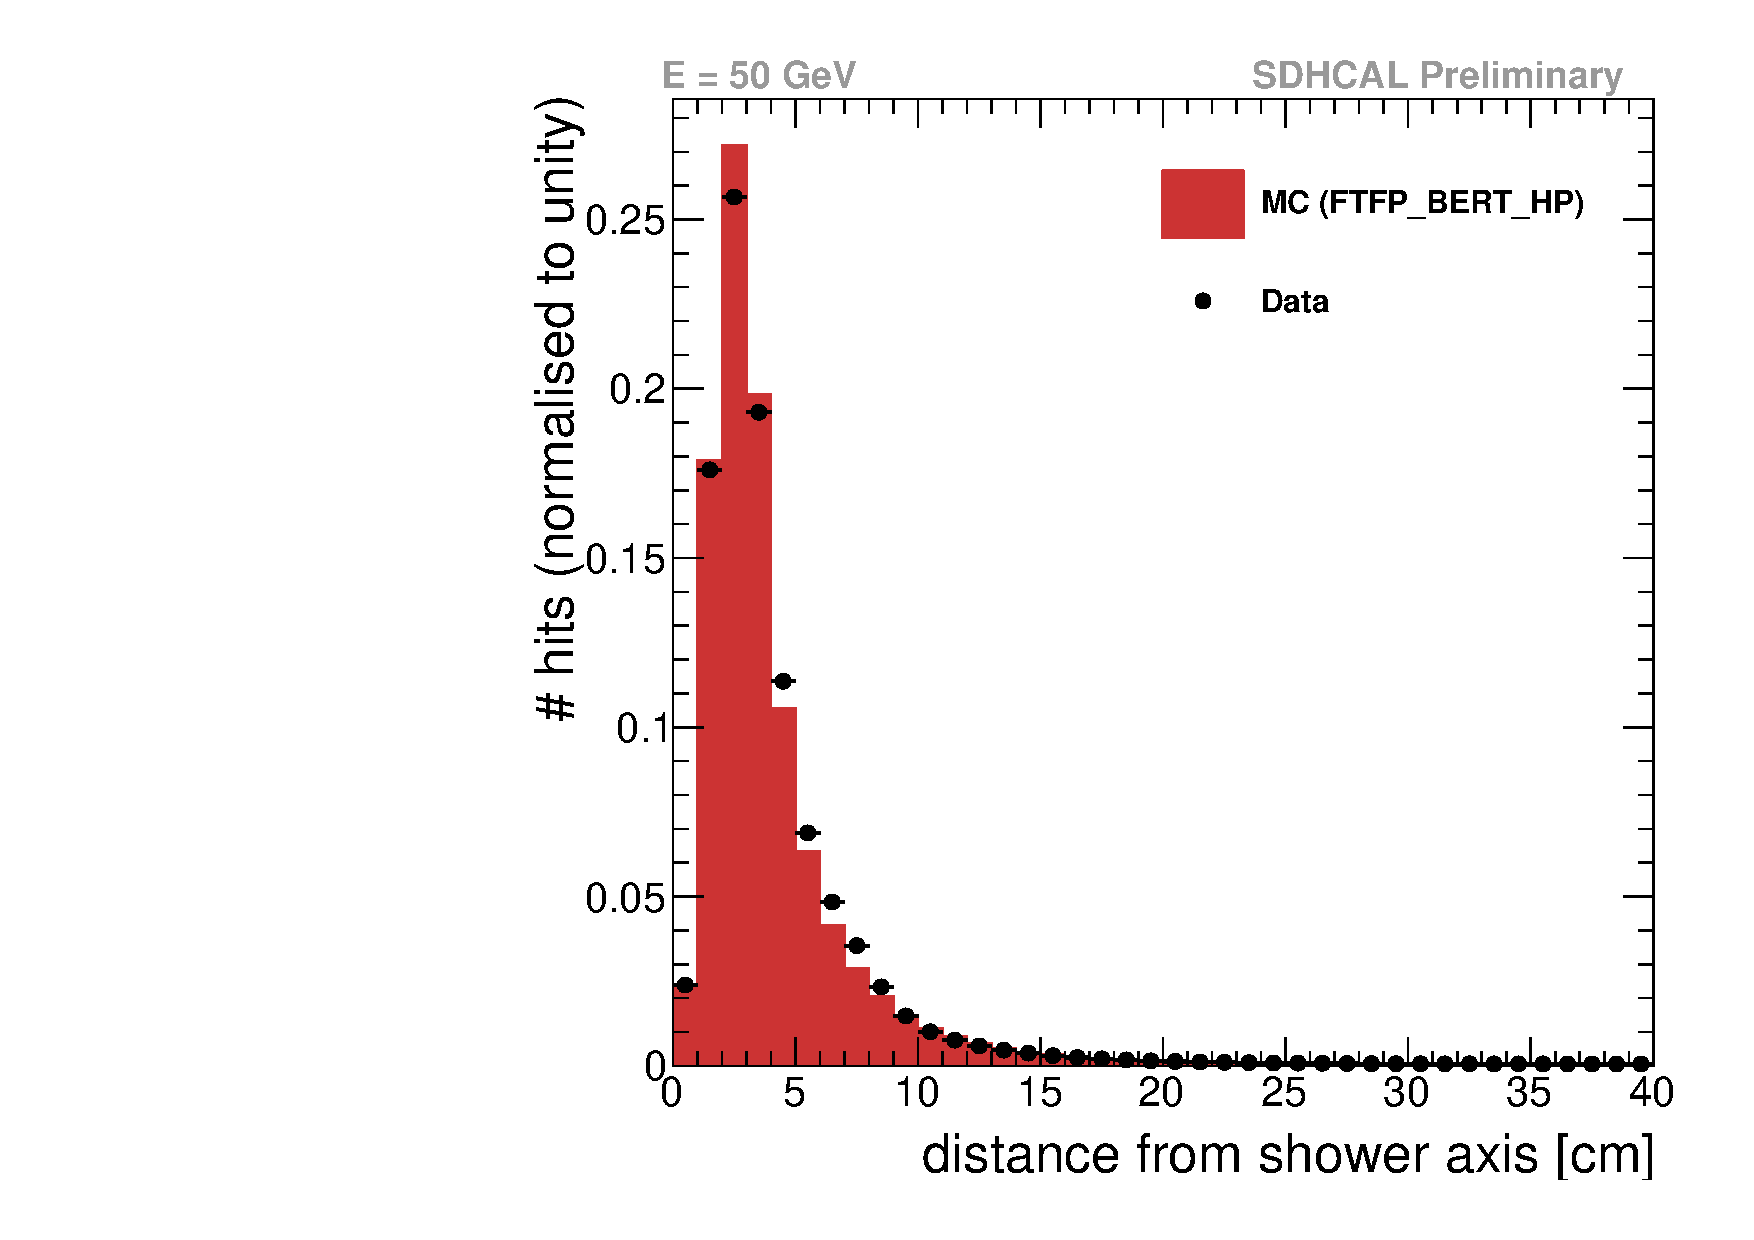
\includegraphics[width=.40\textwidth]{Shower/figs/radProf_e-_50GeV_AugSep2012.pdf}
%%   \caption{Profil transversal de gerbes électromagnétiques à 20 (à gauche) et 50 $GeV$ (à droite) pour les données (cercles noirs) et une simulation réalisée avec liste physique FTFP\_BERT\_HP (histogramme plein).}
%%   \label{fig.rad_e-}
%% \end{figure}
%% \begin{figure}[!ht]
%%   \centering
%%   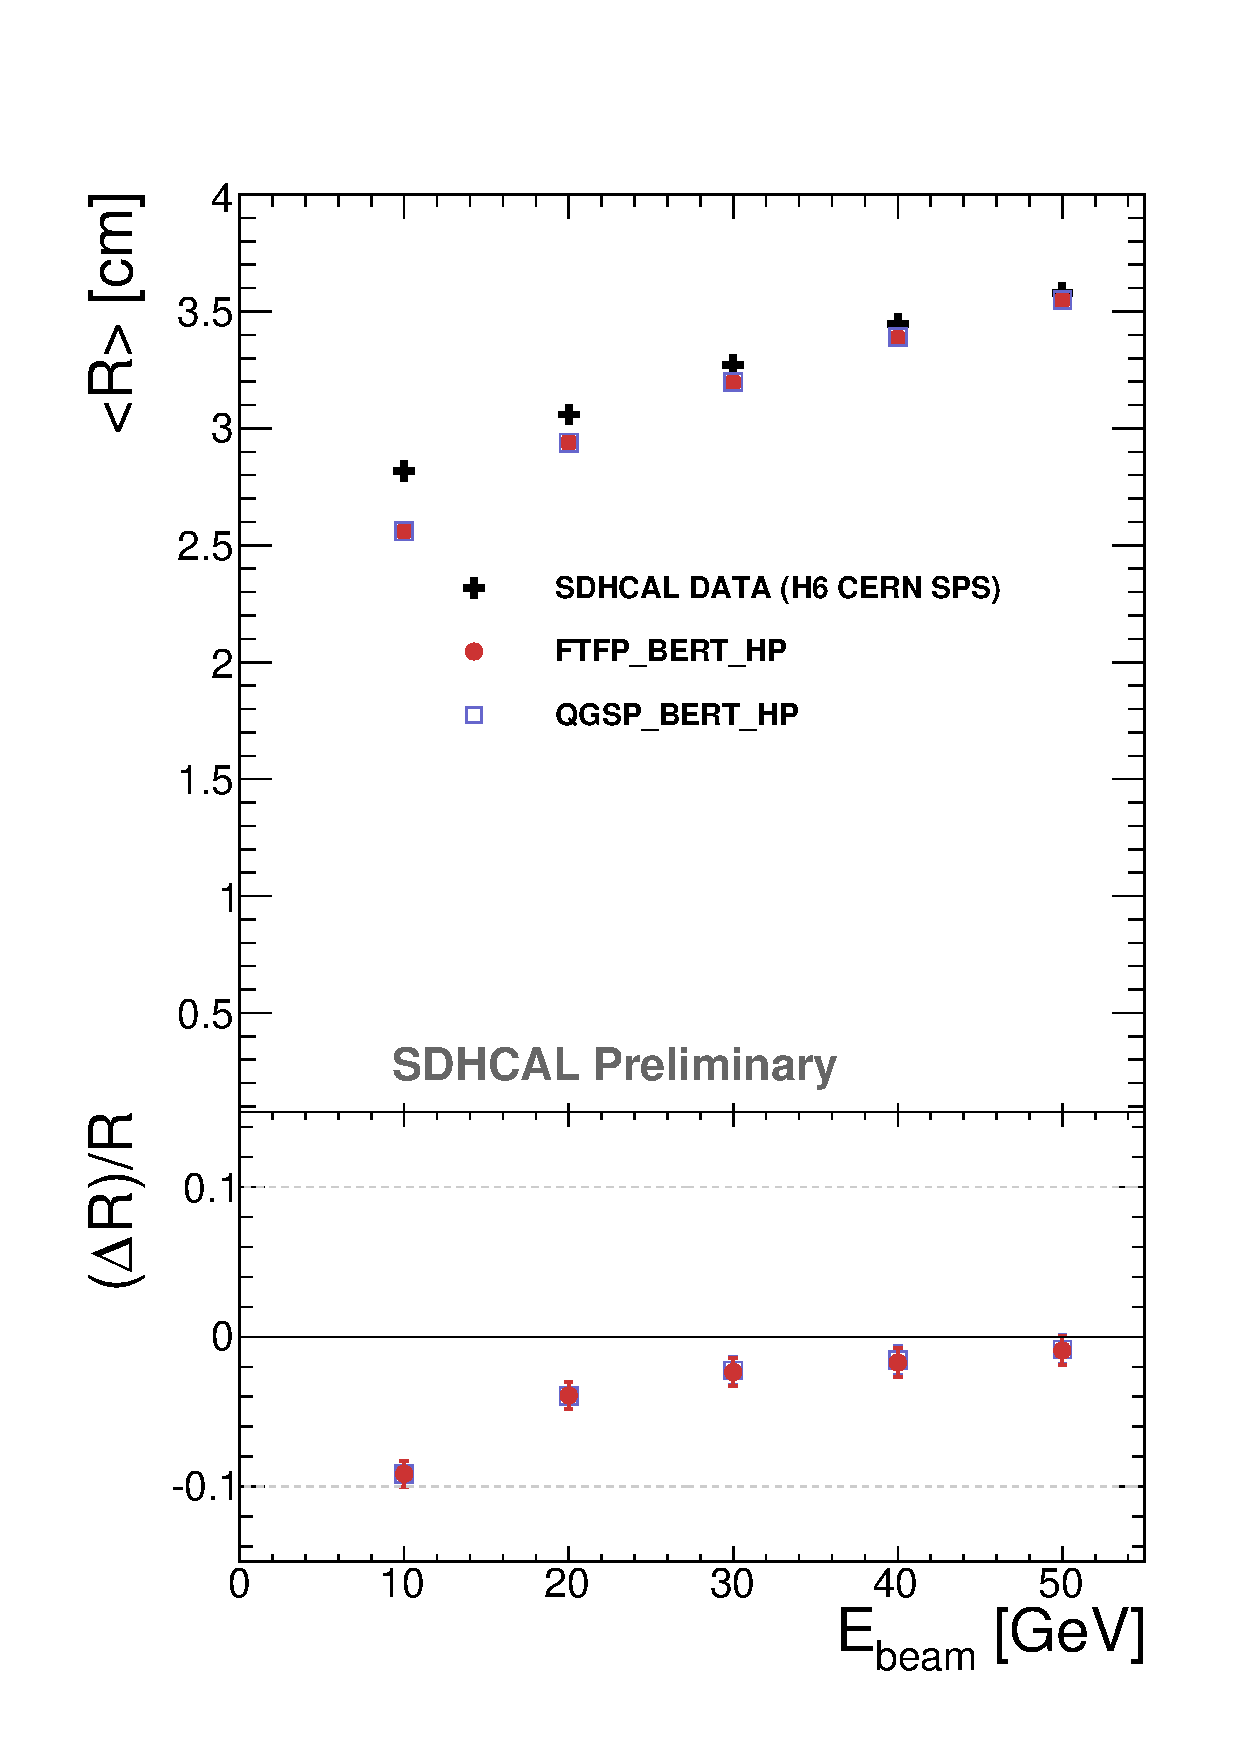
\includegraphics[width=.4\textwidth]{Shower/figs/RADELECTRON.pdf}
%%   \caption{Valeur moyenne et déviation relative du profil transversal pour des gerbes électromagnétiques en fonction de l'énergie du faisceau.}
%%   \label{fig.rad_e-_ebeam}
%% \end{figure}
%\chapter{}
%% \label{app.proton_track}
%% \begin{figure}[!ht]
%%   \centering
%%   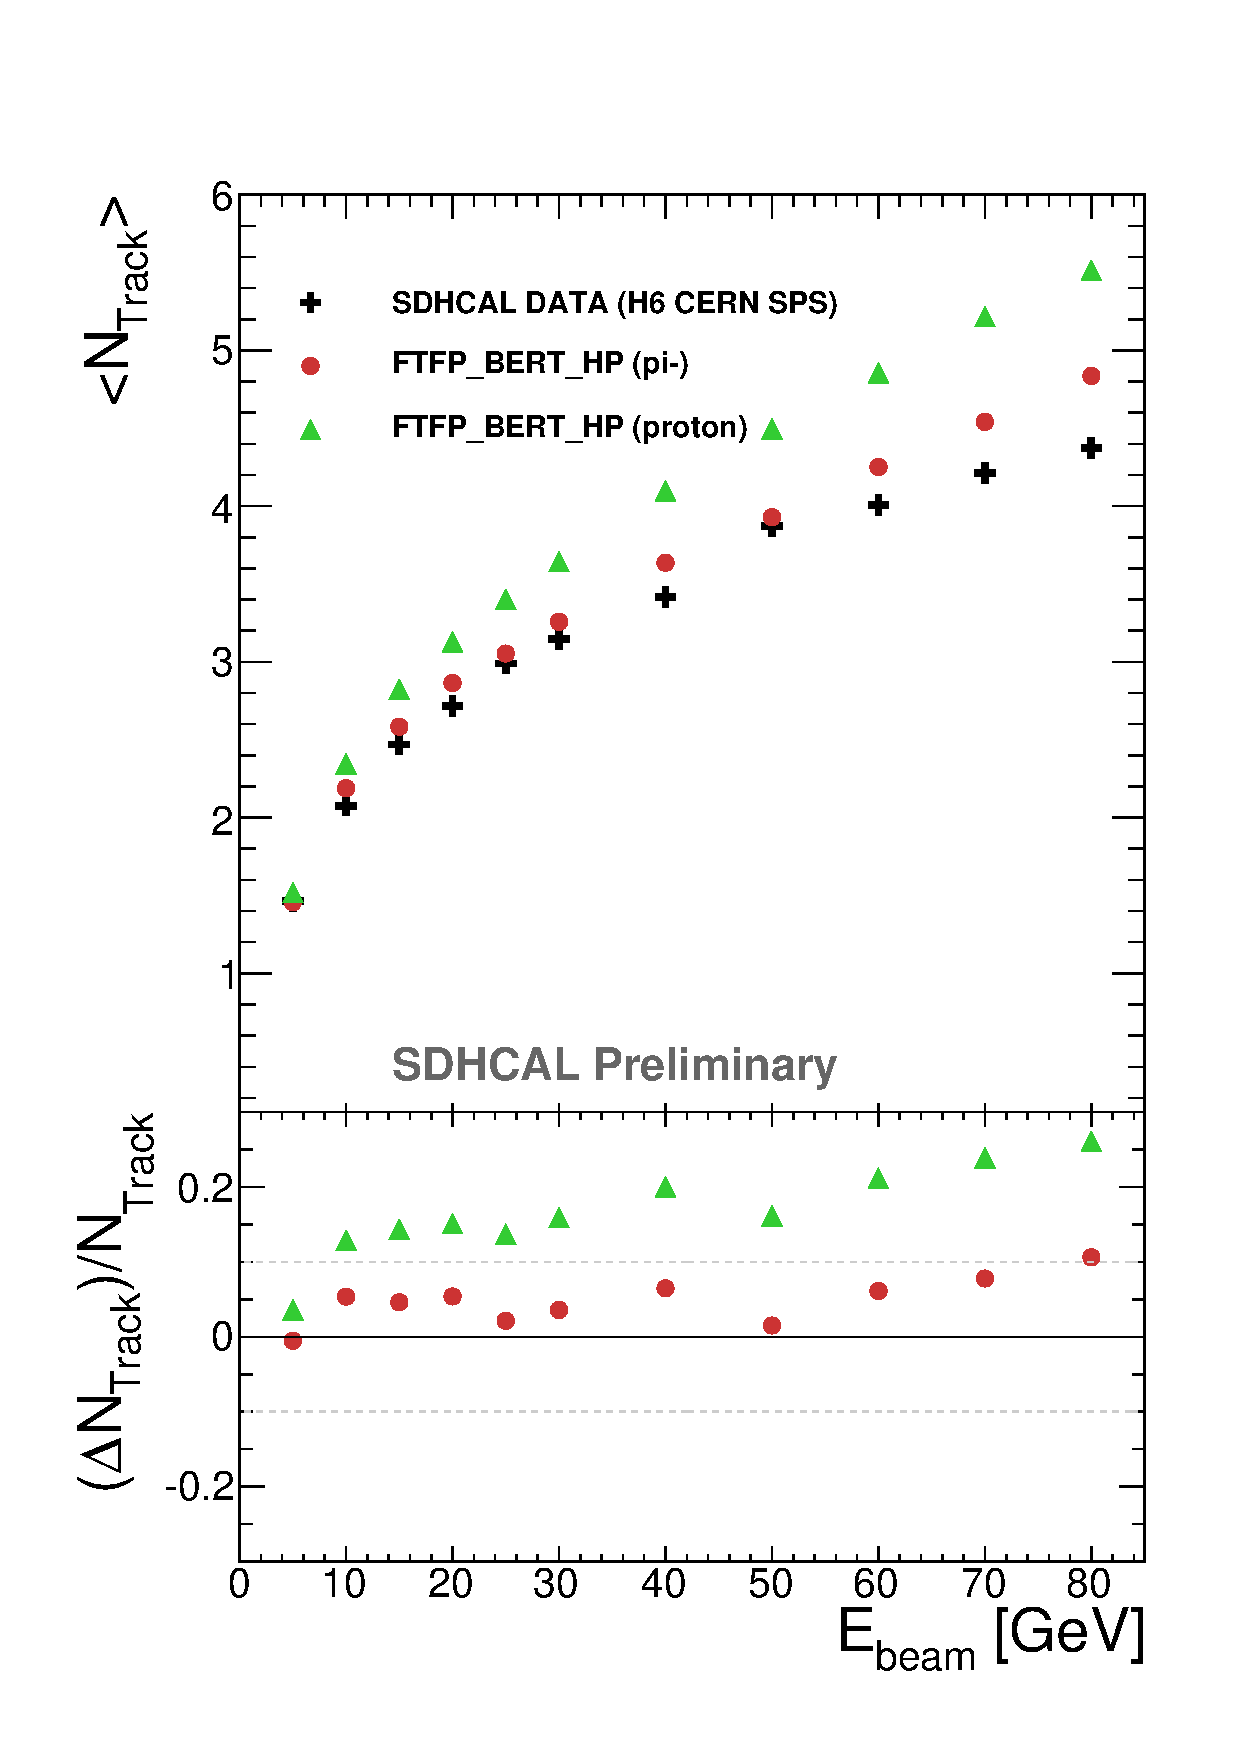
\includegraphics[width=.45\textwidth]{Shower/figs/NTRACKPROTON_FTFP.pdf}
%%   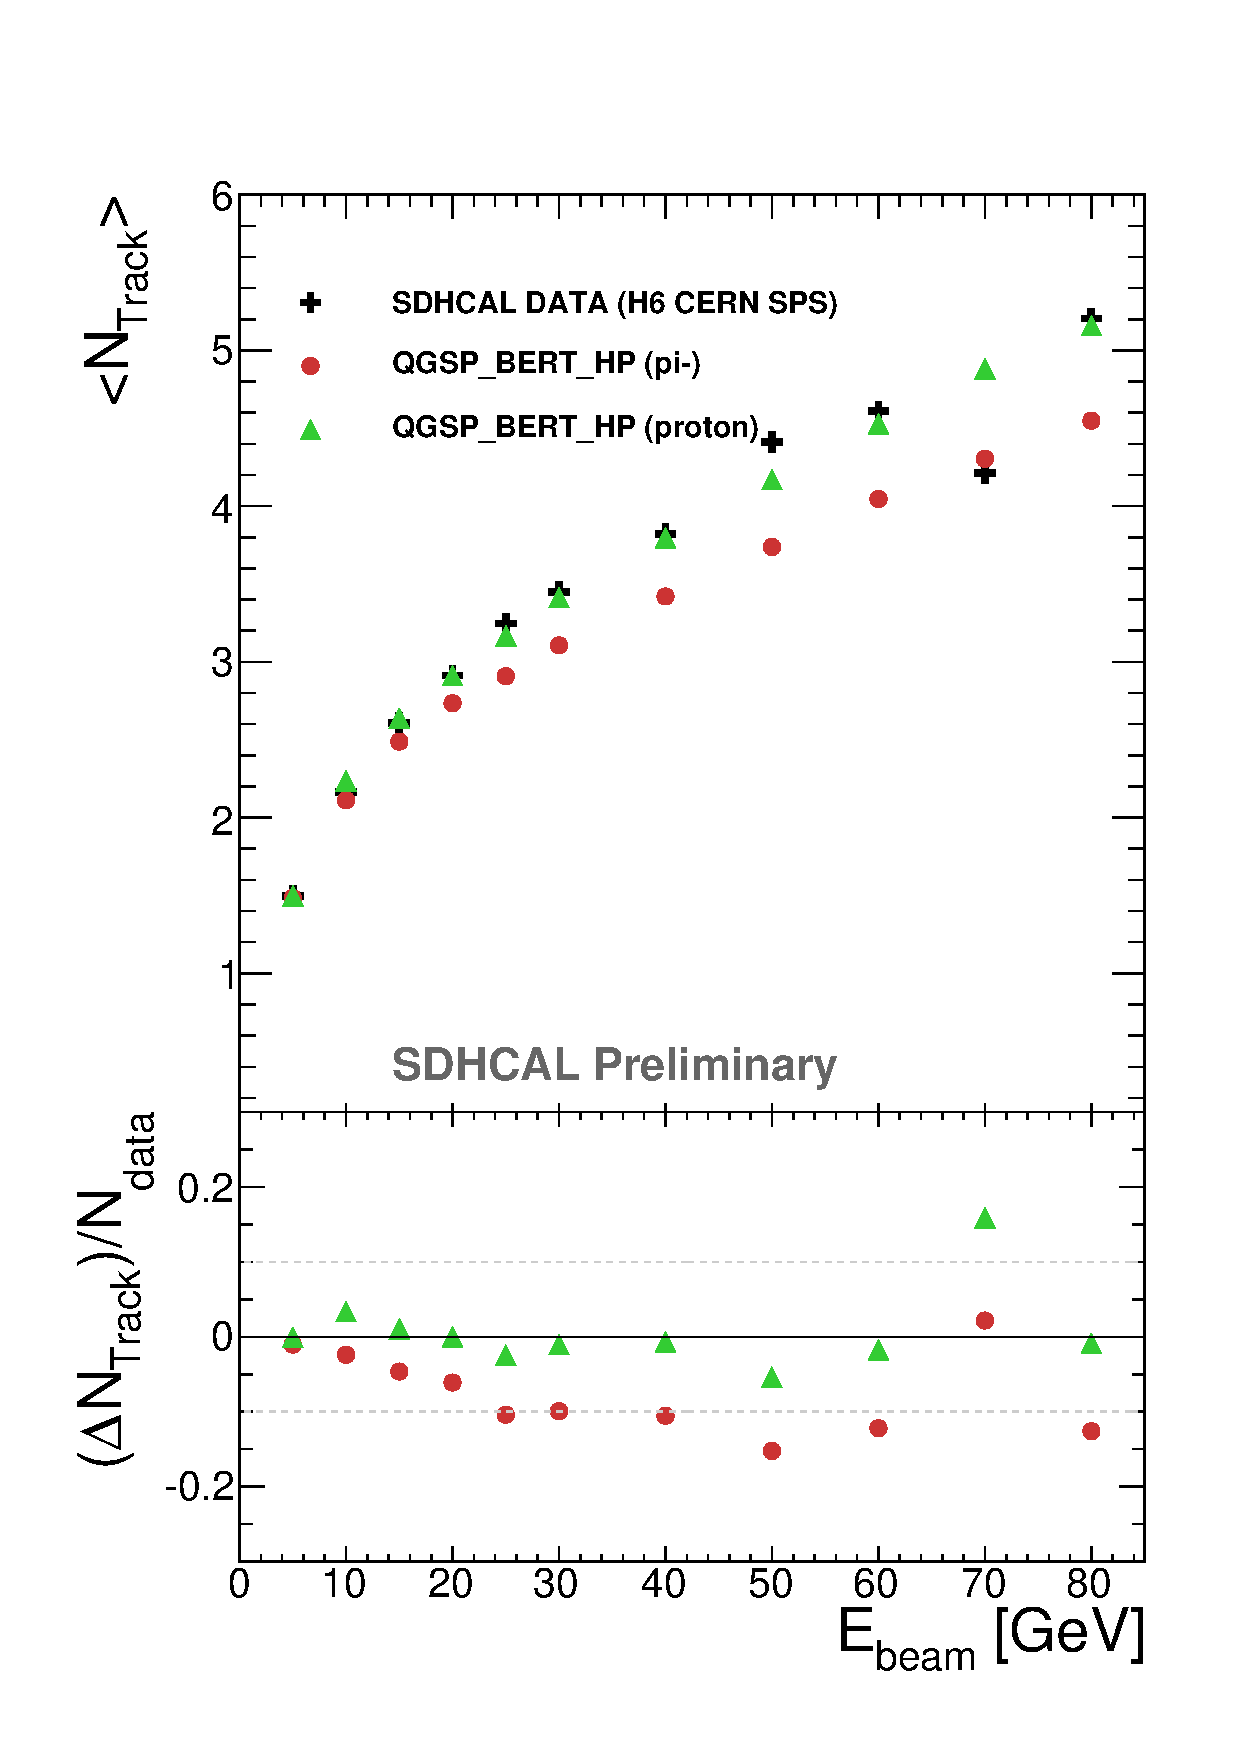
\includegraphics[width=.45\textwidth]{Shower/figs/NTRACKPROTON_QGSP.pdf}
%%   \caption{Moyenne du nombre de traces reconstruites avec la Transformée de Hough en fonction de l'énergie pour les données, des simulations de pions et de protons avec les listes FTFP\_BERT\_HP (à gauche) et QGSP\_BERT\_HP (à droite). Les déviations relatives sont aussi présentées.}
%%   \label{fig.ntrack_proton_ebeam}
%% \end{figure}

%% \begin{figure}[!ht]
%%   \centering
%%   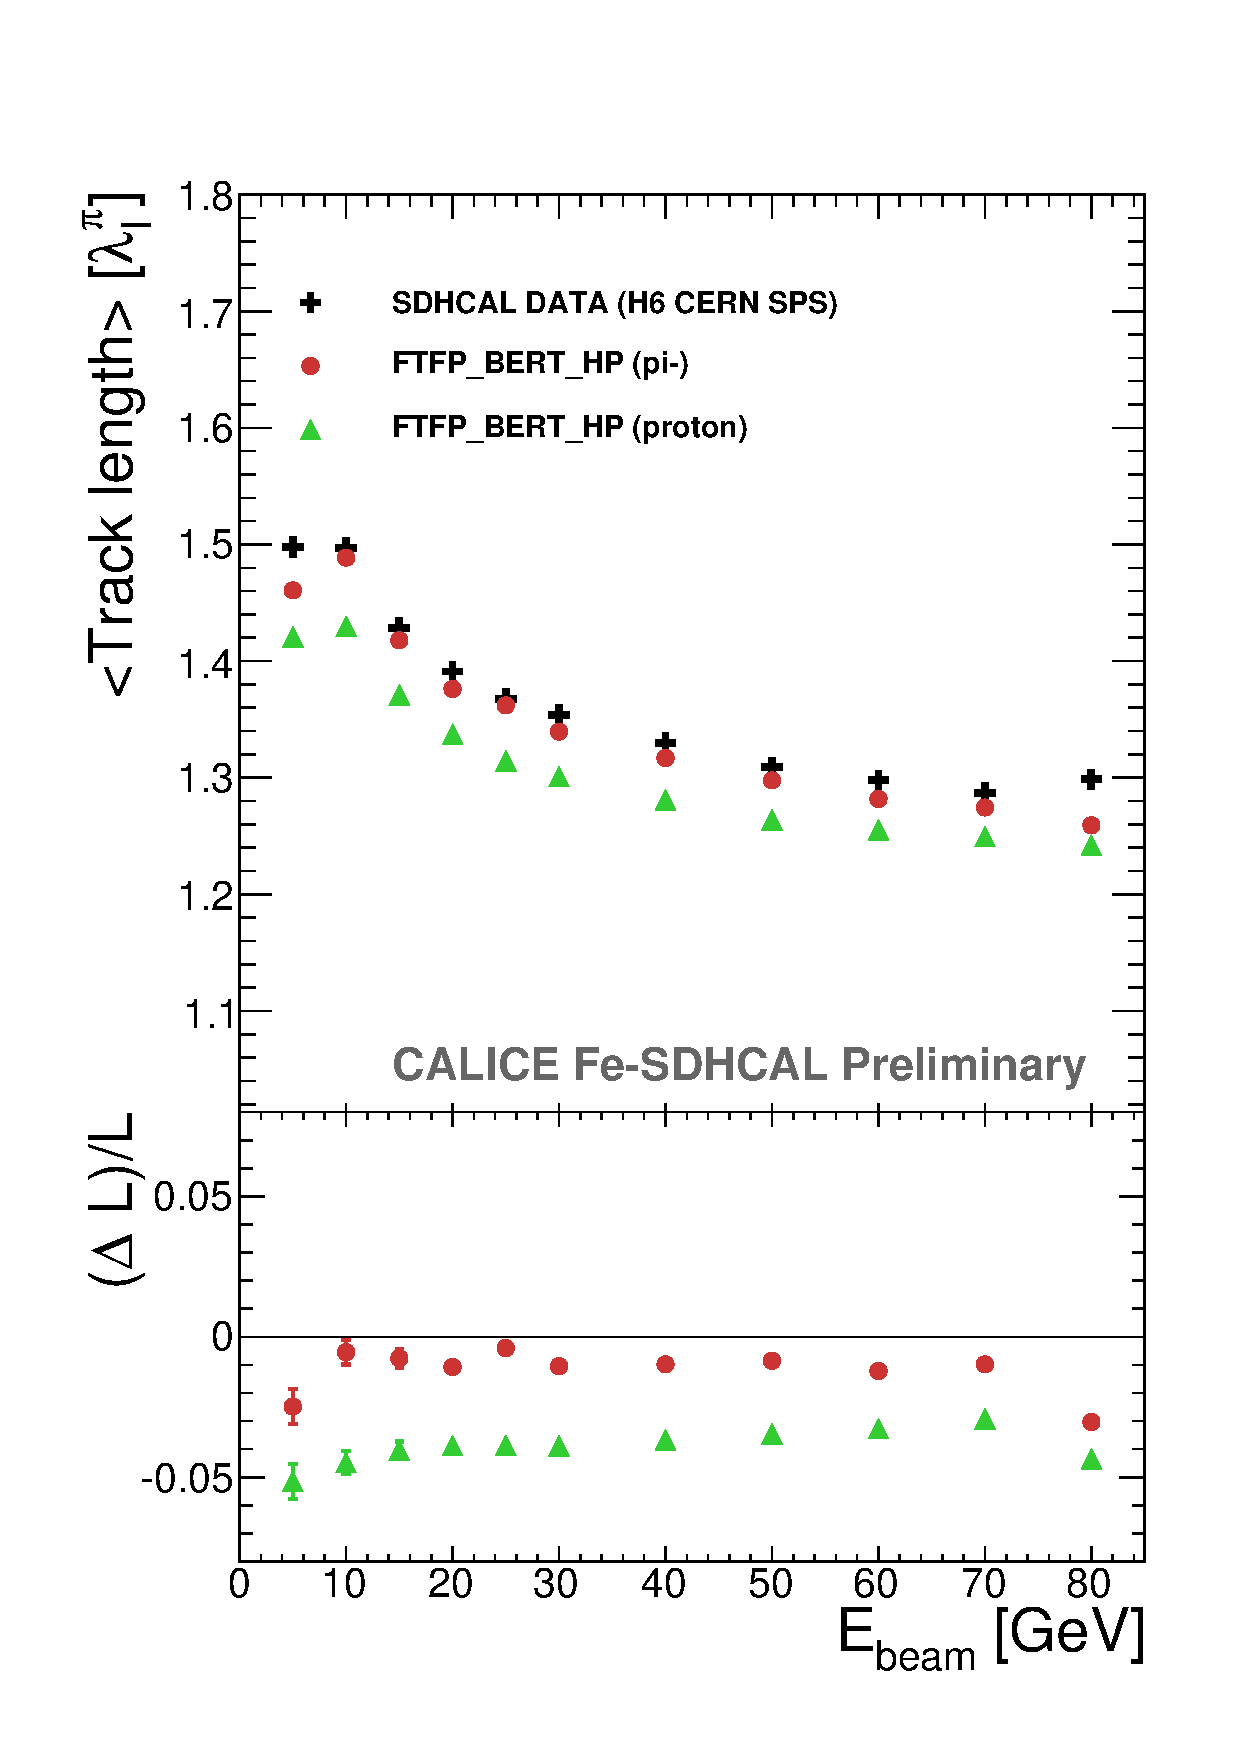
\includegraphics[width=.45\textwidth]{Shower/figs/TRACKLENGTHPROTON_FTFP.pdf}
%%   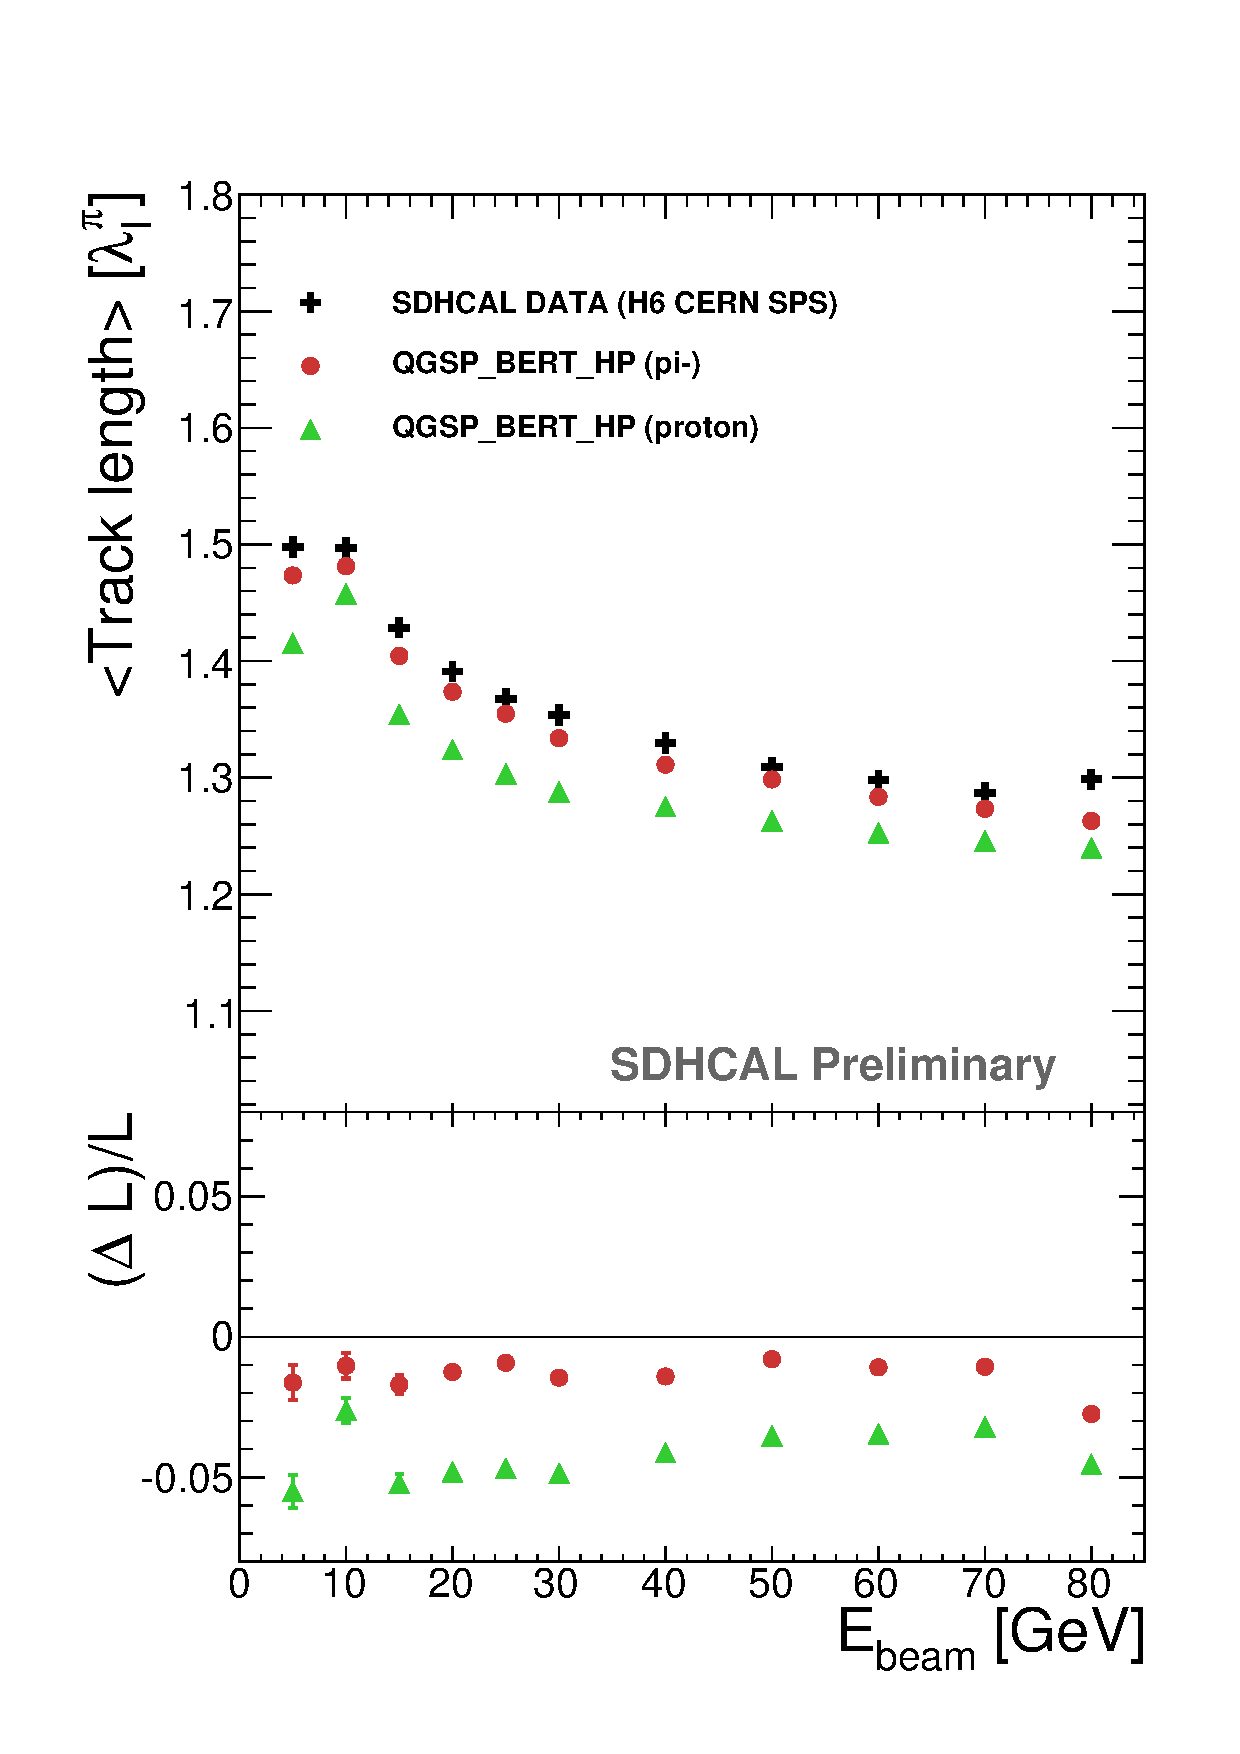
\includegraphics[width=.45\textwidth]{Shower/figs/TRACKLENGTHPROTON_QGSP.pdf}
%%   \caption{Moyenne de la longueur des traces reconstruites avec la Transformée de Hough en fonction de l'énergie pour les données, des simulations de pions et de protons avec les listes FTFP\_BERT\_HP (à gauche) et QGSP\_BERT\_HP (à droite). Les déviations relatives sont aussi présentées.}
%%   \label{fig.tracklength_proton_ebeam}
%% \end{figure}

%% \begin{figure}[!ht]
%%   \centering
%%   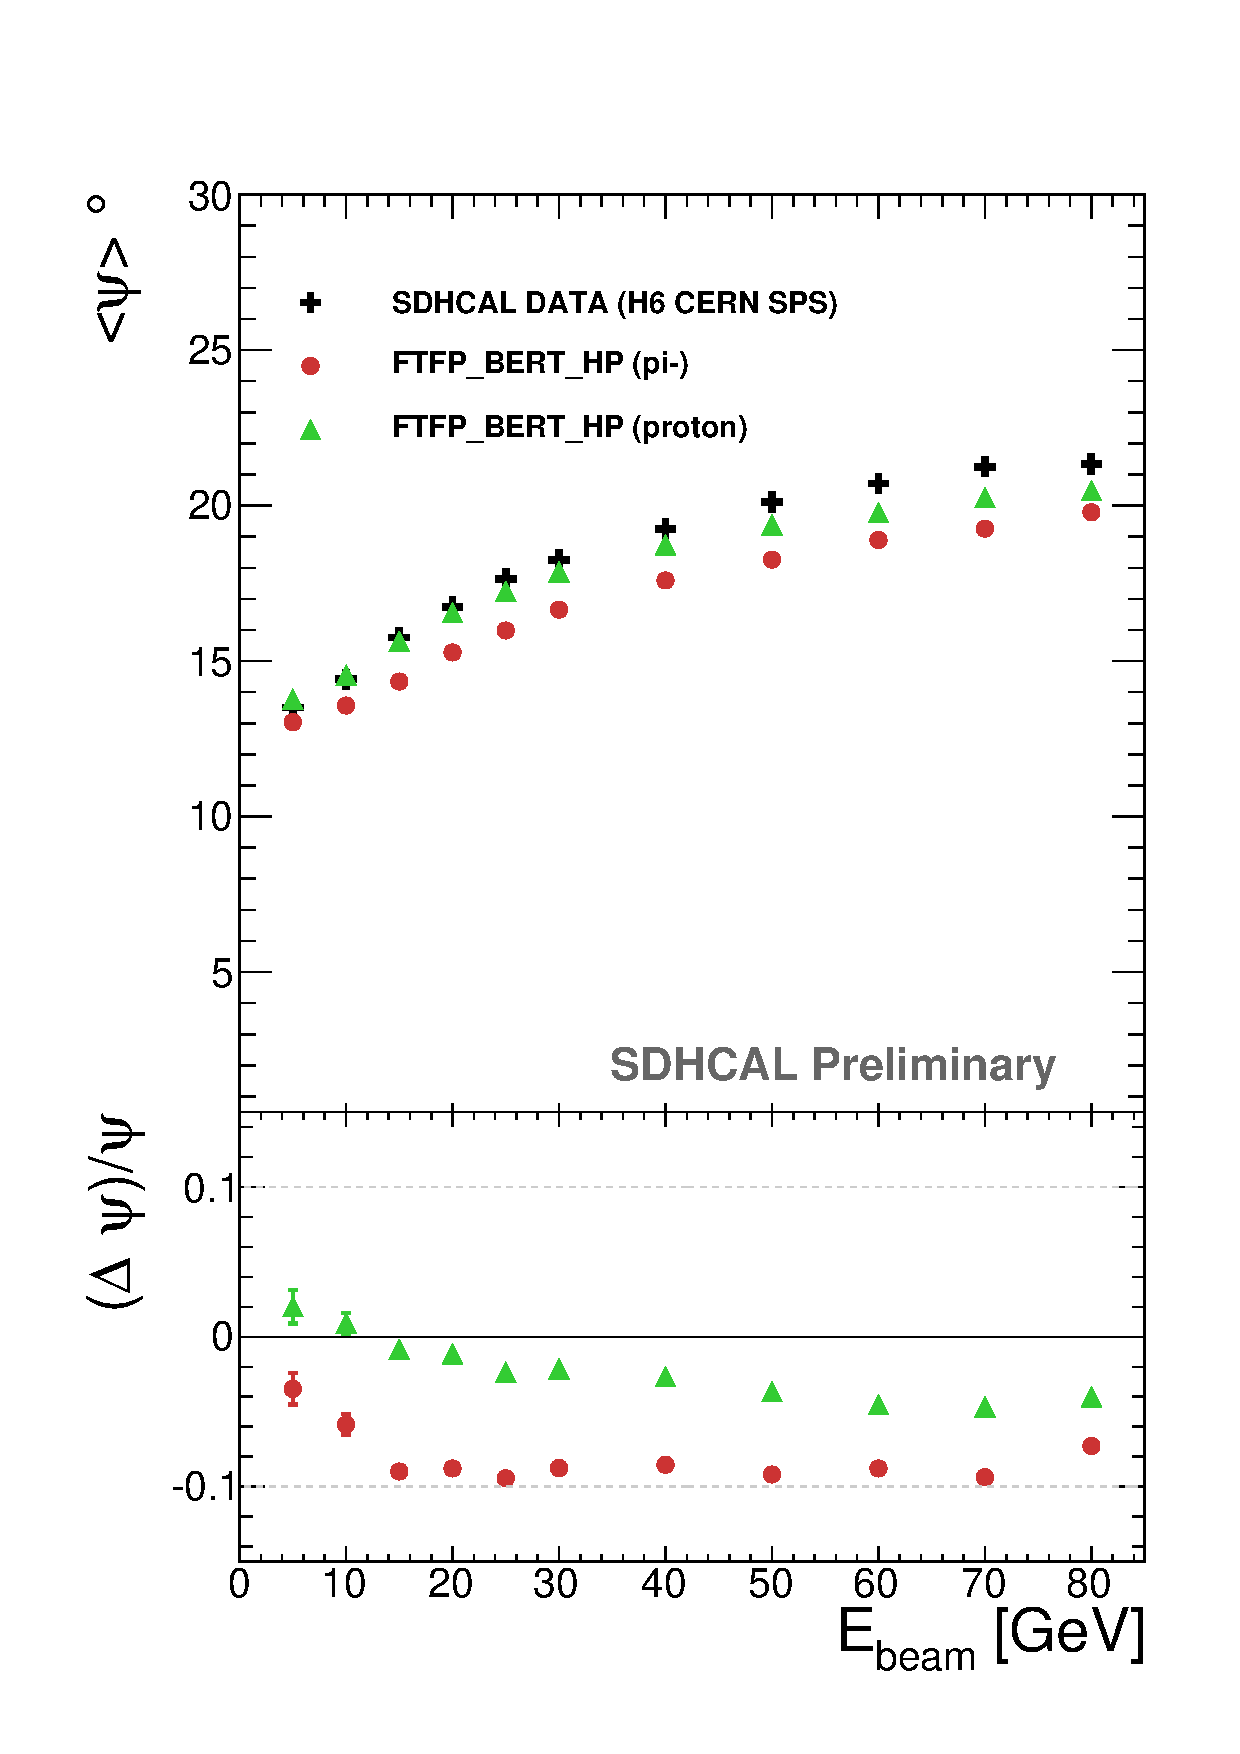
\includegraphics[width=.45\textwidth]{Shower/figs/TRACKANGLEPROTON_FTFP.pdf}
%%   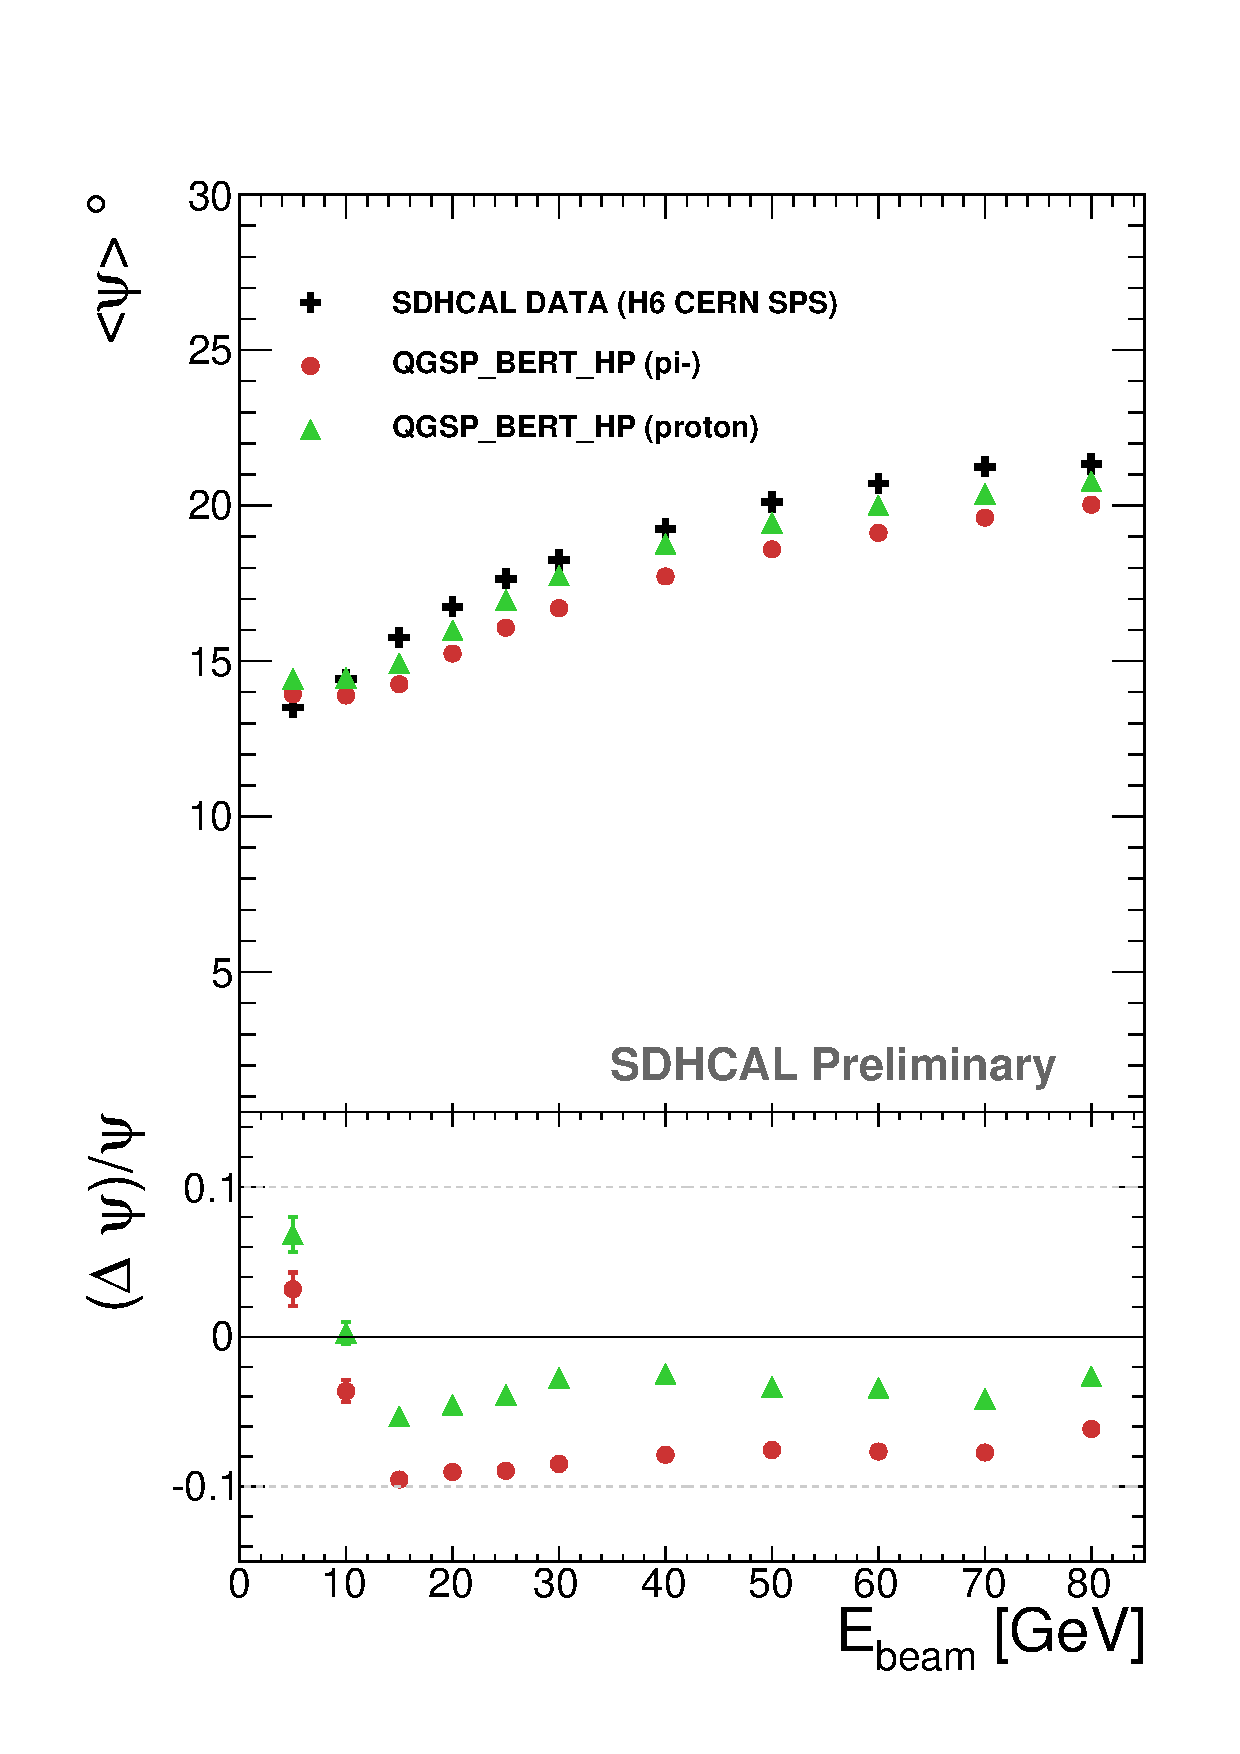
\includegraphics[width=.45\textwidth]{Shower/figs/TRACKANGLEPROTON_QGSP.pdf}
%%   \caption{Moyenne des angles entre les traces reconstruites et l'axe des cascades en fonction de l'énergie pour les données, des simulations de pions et de protons avec les listes FTFP\_BERT\_HP (à gauche) et QGSP\_BERT\_HP (à droite). Les déviations relatives sont aussi présentées.}
%%   \label{fig.trackangle_proton_ebeam}
%% \end{figure}
\end{appendix}
